%     WORK IN PROGRESS %
\documentclass[11pt,a4paper,twoside, draft]{article}%draft wieder rausnehmen
%\documentclass[11pt,a4paper,twoside]{article}
\usepackage[a4paper, bindingoffset=0.5cm, hmargin={2.5cm, 2.5cm},vmargin={2.5cm, 2.5cm}]{geometry}
\usepackage[T1]{fontenc} 
\usepackage[utf8]{inputenc} 
\usepackage[ngerman,english]{babel} 
\usepackage{mathptmx} 
\usepackage{mathtools}
\usepackage{amsmath}
\usepackage{amssymb}
\usepackage{bbm}
\usepackage{latexsym}
\usepackage{nicefrac}
\usepackage{comment}
\usepackage{fp}
\usepackage{cite}
\usepackage{url}
\usepackage{float}
\usepackage{caption}
%\usepackage[ngerman, num]{isodate}
\usepackage[ngerman]{datetime}
\newtheorem{Tm}{Satz}[section]
\newtheorem{Tms}{Satz}[subsection]
\newtheorem{Lm}[Tm]{Lemma}
\newtheorem{Df}[Tm]{Definition}
\newtheorem{Lms}[Tms]{Lemma}
\newtheorem{Dfs}[Tms]{Definition}
\newtheorem{Bsps}[Tms]{Beispiel}
\newtheorem{Bsp}[Tm]{Beispiel}
%Abbildungen sollen Abb. genannt werden und nicht Figure
\newdateformat{myformat}{\THEDAY{. }\monthnamengerman[\THEMONTH], \THEYEAR}
\addto{\captionsngerman}{%
  \renewcommand*{\contentsname}{Inhalt}
  \renewcommand*{\listfigurename}{Abbildungen}
  \renewcommand*{\figurename}{Abb.}
}
\addto{\captionsenglish}{%
  \renewcommand*{\contentsname}{Inhalt}
  \renewcommand*{\listfigurename}{Abbildungen}
  \renewcommand*{\figurename}{Abb.}
}

%\ifpdf %%Einbindung von Grafiken mittels \includegraphics{datei}
	\usepackage[pdftex]{graphicx} %%Grafiken in pdfLaTeX
%\else
%	\usepackage[dvips]{graphicx} %%Grafiken und normales LaTeX
%\fi
%\usepackage[hang,tight,raggedright]{subfigure} %%Teilabbildungen in einer Abbildung
%\usepackage{pst-all} %%PSTricks - nicht verwendbar mit pdfLaTeX
\usepackage{fancyhdr}
\pagestyle{fancy}
%% Zeilenabstand %%%%%%%%%%%%%%%%%%%%%%%%%%%%%%%%%%%%%%%%%%%%
%\usepackage{setspace}
%\singlespacing        %% 1-zeilig (Standard)
%\onehalfspacing       %% 1,5-zeilig
%\doublespacing        %% 2-zeilig

%absaetze
\parindent0cm
\parskip0.2cm

%\usepackage[pdftex,bookmarks=true,colorlinks=true,
%        linkcolor=black,
%        citecolor=black,
%        filecolor=black,
%        pagecolor=black,
%        urlcolor=black,
%        bookmarks=true,
%        bookmarksopen=true,
%        bookmarksopenlevel=3,
%        plainpages=false,
%        pdfpagelabels=true]{hyperref}


% Title Page

\usepackage{todonotes}
\usepackage{mwe}

\begin{document}
%% Abschnittsueberschriften auf rechter Seite(odd) links
%% - Abschnitt - Seitenzahlen aussen
\lhead[\fancyplain{}{\thepage}]{\fancyplain{}{\rightmark}}
%% Kapitelueberschriften auf linker Seite(even) rechts
%% - Kapitel - Seitenzahlen aussen
\rhead[\fancyplain{}{\leftmark}]{\fancyplain{}{\thepage}}
\cfoot{}
\pagenumbering{roman}
\begin{titlepage}
\begin{center}
\vspace*{0.65cm}
\huge\pagenumbering{arabic}
\setcounter{page}{1}
\hspace*{-0.73cm}
\textbf{Das Matrix-Tree-Theorem}\\
\vspace*{2.2cm}

\begin{figure}[h]
	\begin{center}
		\hspace*{-0.73cm}
		
\includegraphics{lmu_siegel}
	\end{center}
\end{figure}
%%
\vspace*{0.5cm}
\Large
\hspace*{-0.73cm}
\hspace*{-0.5cm}Bachelorarbeit der Fakultät für Mathematik\\
\vspace*{0.1cm}
\hspace*{-0.73cm}
\hspace*{-0.5cm}der\\
\vspace*{0.1cm}
\hspace*{-0.73cm}
\hspace*{-0.5cm}Ludwig-Maximilians-Universität München\\
%%
%\vspace*{3.7cm}
\vspace*{3.5cm}
\large
\hspace*{-0.73cm}
\hspace*{-0.8cm} vorgelegt von\\
\vspace*{0.1cm}
\hspace*{-0.73cm}
\hspace*{-0.7cm}\Large \textbf{Christopher Mann}\\
\vspace*{0.15cm}
\large
\hspace*{-0.73cm}
\hspace*{-0.8cm} geboren in Freising\\
\vspace*{1.5cm}
\vspace*{0.4cm}Betreuer: \textbf{Prof. Dr. Konstantinos Panagiotou}\\
\vspace*{1cm}
\hspace*{-0.73cm}
\hspace*{-0.43cm}München, den \myformat\today\\
\end{center}
\end{titlepage}


%
%%%%%%%%%%%%%%%%%%%%%%%%%%%%%%%%%%%%%%%%%%%%%%%%%%%%%%%%%%%%%%%%%%%%%%
%
\clearpage{\pagestyle{empty}\cleardoublepage}
%
%%%%%%%%%%%%%%%%%%%%%%%%%%%%%%%%%%%%%%%%%%%%%%%%%%%%%%%%%%%%%%%%%%%%%%


%\thispagestyle{empty}

\cleardoublepage

\pagestyle{plain}
\pagenumbering{arabic} 
\setcounter{page}{1}

\tableofcontents
\cleardoublepage

\section{Einleitung}
%Graphentheorie spielt in allen MINT-Fächern eine Rolle. 
%Sie ist daher ein besonders zukunftsweisender Zweig der Mathematik. 
%Diese Arbeit beschäftigt sich mit sogenannten Matrix-Tree-Theorems.  
Schon 1847 schrieb Kirchhoff in seiner Arbeit "Ueber[sic!] die Auflösung der Gleichungen, auf welche man bei der Untersuchung der linearen Verteilung galvanischer Ströme geführt wird;"\cite{kirchhoff_1847} als erster implizit über den Zusammenhang zwischen Matrizen und der Anzahl von Spannbäumen von Graphen - explizit über Systeme von beliebig miteinander verbundenen Drähten und Gleichungen für die elektrischen Stromstärken in diesem System.
In der Graphentheorie sind Matrix-Tree-Theorems neben anderen Methoden, wie Prüfer-codes, beliebte Werkzeuge um die Anzahl der Spannbäume eines Graphen zu ermitteln.
Das wohl berühmteste, nach Kirchhoff benannte Matrix-Tree-Theorem wird oft als das Matrix-Tree-Theorem bezeichnet, wobei es auch noch andere Versionen, wie Tuttes Matrix-Tree-Theorem für gerichtete Multigraphen, dessen Beweis auch Teil dieser Arbeit sein wird, gibt.
Aber auch außerhalb der reinen Mathematik und der Theorie über elektrische Schaltkreise finden Matrix-Tree-Theorems ihre Anwendung.\\
So wird das Matrix-Tree-Theorem zum Beispiel in der Quantenphysik genutzt \cite{giovannetti_severini_2013}.
In der Chemie gibt es einen Zusammenhang zwischen Spannbäumen und der Complexität von Molekülen \cite{janezic_2015}.
Auch in der Informatik kann man Matrix-Tree-Theorems zum Beispiel dafür benutzen, die Anzahl von Spannbäumen von Netzwerken - die man als Graphen betrachen kann - zu berechnen, um dann Rück\-schlüsse über die Stabilität dieser Netzwerke zu ziehen \cite{yakoubi_2019}.
Das Anwendungsspektrum von Matrix-Tree-Theorems ist also vielseitig.
In dieser Arbeit werden wir uns zwei Matrix-Tree-Theorems erschließen und damit im Anschluss die Anzahl der Spannbäume von Graphen einiger Klassen bestimmen.


\section{Grundlegende Definitionen und Notationen}
Wir beginnen damit, ein paar wichtige Begriffe und Notationen einzuführen, die wir später häufiger benutzen werden.
In einem Matrix-Tree-Theorem wird immer ein Zusammenhang zwischen bestimmten Matrizen und den Spannbäumen eines Graphen beschrieben. Daher bieten sich die folgenden zwei Definitionen an, von denen wir eine für ungerichtete und die andere für gerichtete Graphen verwenden werden.
\begin{Df}\textbf{Laplacematrix}\\
Für einen Graphen $G=(V,E)$ indizieren wir die Zeilen und Spalten einer Matrix mit den Knoten von G. Die Matrix mit den Einträgen
$$
l_{ij}=
\begin{cases}
 d(i),\, \, falls\,\, i=j,\\
 (-1), \, \, falls \,\, ij \in E,\\
 0, \,\, sonst.
\end{cases}
$$
nennen wir die Laplacematrix $L(G)$ des Graphen $G$.
\end{Df}
Für einen Knoten $i$ bezeichnen wir mit $d^{-}(i)$ seinen Ausgangsgrad.
\begin{Df}\textbf{Kirchhoffmatrix}\\
 Für einen gerichteten Multigraphen $D$ mit Knoten $1,..,n$ definieren wir die Kirchhoffmatrix $K(D)$ wie folgt:\\
 $$
k_{ij}=
\begin{cases}
 d^{-}(i),\, \, falls\,\, i=j,\\
 (-m), \, \, wobei \,\, m \,\, die\, Anzahl\, der\, Kanten\, von\,\, i\,\, nach \,\,j\,\, ist.
\end{cases}
$$
Wobei wir wieder die Zeilen und Spalten mit den Knoten von $D$ indiziert haben.\\
Nachdem wir in Tuttes Matrix-Tree-Theorem eine Zeile und Spalte streichen müssen, bezeichnen wir mit $K_{\bar{i}}(D)$ die Matrix, die entsteht, wenn man aus $K(D)$ die $i$-te Zeile und Spalte löscht.
\end{Df}
Im Verlauf dieser Arbeit werden wir immer wieder die Anzahl der Spannbäume eines Graphen ausrechnen, daher verwenden wir $\mathit{k}(G)$ als die Anzahl der Spannbäume eines beliebigen Graphen $G$.
\todo[inline, color=yellow]{Stand jetzt werde ich die Definitionen als solche hervorheben, Notation jedoch im Fließtext unterbringen, passt das so?-JA}

\section{Das Matrix-Tree-Theorem}

Nachdem wir genügend Vorarbeit geleistet haben, können wir mit dem wichtigsten Teil dieser Arbeit anfangen, dem Beweis der Matrix-Tree-Theorems selbst. Wir beweisen zuerst eine Version für gerichtete Multigraphen, bevor wir uns der Version für ungerichtete Graphen als einem Spezialfall davon widmen.

\subsection{Tuttes Matrix-Tree-Theorem}
Um die Version des Matrix-Tree-Theorems für gerichtete Multigraphen und den dazugehörigen Beweis zu verstehen, müssen wir zuerst den Begiff der Aboreszenz einführen.
Als Aboreszenz aus einem Knoten bezeichnen wir einen gerichteten Baum, der diesen Knoten als Wurzel hat, wobei die Kanten von der Wurzel ausgehen.\\
Nun können wir ein Matrix-Tree-Theorem für gerichtete Multigraphen formulieren:
\begin{Tms}[Tuttes Matrix-Tree-Theorem]
\sloppypar
Sei $D$ ein gerichteter Multigraph mit Kirchoffmatrix $K(D)$. Die Anzahl der Aboreszenzen aus einem Knoten $i$ ist gleich der $\det(K_{\bar{i}}(D))$.
\par
\end{Tms}
Um das zu beweisen lassen wir uns von \cite{bang-jensen_2009} inspirieren.
Also zeigen wir zuerst folgendes Lemma:
\begin{Lms}
Sei $D$ ein gerichteter Multigraph mit maximalem Eingangsgrad $=1$ und $i$ ein Knoten in $D$.\\
Dann hat $D$ maximal eine Aboreszenz mit Wurzel $i$. Desweiteren ist $\det(K_{\bar{i}}(D)) \in \{0,1\}$
und genau dann, wenn $D$ eine Aboreszenz mit Wurzel $i$ besitzt, ist $\det(K_{\bar{i}}(D)) = 1$.
\label{L1}
\end{Lms}
\textbf{Beweis von Lemma ~\ref{L1}:}\\
Wir nehmen zuerst an, dass $D$ eine Aboreszenz mit Wurzel $i$ hat.\\
Da der maximale Eingangsgrad $=1$ ist, schließen wir, dass für jeden Knoten außer $i$, die eine eingehnende Kante in dieser Aboreszenz enthalten ist. \\
Weil das Vertauschen von Zeilen einer Matrix deren Determinante nicht ändert, dürfen wir annehmen, dass $i=1$ ist und die übrigen Knoten in der Reihenfolge einer Breitensuche durchnummeriert sind.\\ 
Dann ist nämlich $K_{\bar{i}}(D)$ eine obere Dreiecksmatrix mit Diagonaleinträgen $=1$, also $\det(K_{\bar{i}}(D)) = 1$.
Jetzt nehmen wir an, dass $D$ keine Aboreszenz mit Wurzel $i$ besitzt.\\
Falls ein anderer Knoten als $i$ Eingangsgrad $=0$ hat, sind die alle Einträge der entsprechenden Spalte von $K_{\bar{i}}(D)$ und damit auch $\det(K_{\bar{i}}(D))$ gleich $0$\\
Deshalb dürfen wir zu guter Letzt annehmen, dass für alle von $i$ verschiedenen Knoten der Eingangsgrad $=1$ ist.\\
Weil $D$ keine Aboreszenz mit Wurzel $i$ besitzt, hat $D$ einen Zyklus, der $i$ nicht enthält.\\
Da aber jeder Knoten $\neq i$ Eingangsgrad $=1$ hat, sind die Spalten, die mit den Knoten in diesem Zyklus korrespondieren, linear abhängig und damit $\det(K_{\bar{i}}(D)) = 0$.\\
Damit haben wir unser Lemma bewiesen.
\begin{flushright} $\Box$ \end{flushright} 

Nun können wir uns dem Beweis von Tuttes Matrix-Tree-Theorem widmen.

\textbf{Beweis von Tuttes Matrix-Tree-Theorem:}
Wir werden die Matrix $K(D)$ in kleinere Matrizen zerlegen und dann mit dem Lemma von oben arbeiten.\\
Bei der Zerlegung in kleinere Matrizen erinnern wir uns an ein Ergebnis aus der linearen Algebra:
Für eine Matrix aus Spalten $c_1,..,c_n$ mit jeweils $n$ Elementen gilt:
\begin{equation}
 \det(c_1,..,(c_i+\prime{c_i}),..,c_n) = \det(c_1,..,c_i,..,c_n) + \det(c_1,..,\prime{c_i},..,c_n)
\end{equation}
\todo[inline, color=blue]{Im folgenden Satz nachm Leerzeichen einfügen dieselben zwischen nxn und Matrix wieder wegmachen, das gehört nämlich zusammen}
Weil sich die einzigen positiven Einträge von $K(D)$ auf der Diagonale befinden und die Spaltensummen alle $=0$ sind, können wir $K(D)$ auf diese Weise in  $s=\prod_{i=1}^nk_{ii}$ $n \times n$-Matrizen $K(D_i), i\in\{1,..,s\}$ zerlegen, indem wir jede Spalte als Summe von $k_{ii}$ Spalten schreiben von denen jede mit einer in $i$ eingehenden Kante korrespondiert.\\
Ohne Beschränkung der Allgemeinheit können wir $i=1$ annehmen.\\
Wir werden jetzt $\det(K_{\bar{1}}(D))$ mithilfe der Matrizen von oben vereinfachen und dann ausrechnen.\\
Hierzu sei $\hat{D}$ der Graph der aus $D$ durch löschen aller in den Knoten $1$ eingehenden Kanten entsteht und $d^{-}(j)$ der Eingangsgrad eines Knoten $j$. Dann folgt:
\begin{equation}
 \det(K_{\bar{1}}(\hat{D})) = \sum_{e_2}^{d^{-}(2)}\det(K_{e_2}(\hat{D}))
\end{equation}
,wobei $K_{e_j}(\hat{D})$ aus $\hat{D}$ durch löschen aller in den Knoten $j$ eingehenden Kanten außer $e_j$ entsteht.\\
Wiederholen wir das für die übrigen Knoten, bekommen wir:
\begin{equation}
  \det(K_{\bar{1}}(\hat{D})) = \sum_{e_2}^{d^{-}(2)}...\sum_{e_n}^{d^{-}(n)}\det(K_{e_n})
\end{equation}
Mit Lemma~\ref{L1} schließen wir, dass genau das die Aboreszenzen mit Wurzel $i$ zählt.\\
Da $\det(K_{\bar{i}}(D))$ aus $K(D)$ durch löschen der mit Knoten $i$ korrespondierenden Zeile und Spalte entstanden ist und wir ohne Beschränkung der Allgemeinheit $i=1$ annehmen durften, gilt:
\begin{equation}
 \det(K_{\bar{1}}(\hat{D}))=\det(K_{\bar{1}}(D))=\det(K_{\bar{i}}(D))
\end{equation}
Das vervollständigt unseren Beweis von Tuttes Matrix-Tree-Theorem.
\begin{flushright} $\Box$ \end{flushright} 


\subsection{Kirchhoffs Matrix-Tree-Theorem}
Nun werden wir das Matrix-Tree-Theorem für ungerichtete Graphen formulieren und beweisen, dass wir auch im weiteren Verlauf dieser Arbeit verwenden werden um die Anzahl der Spannbäume für verschiedene Graphenklassen zu bestimmen.
\begin{Tms}[Kirchoffs Matrix Tree Theorem]
Sei $G$ ein ungerichteter Graph und $L_n$  die dazugehörige Laplacematrix. 
Dann gilt:
% Bis hier Text ohne Einrückung
\par
\begingroup
\leftskip=20pt% Parameter anpassen
\rightskip=20pt
\noindent %ab hier der Text, der eingerückt werden soll
(1) Die Anzahl der Spannbäume von $G$ gleich einem beliebigen Kofaktor von $L_n$.\\
(2) Die Anzahl der Spannbäume von $G$ gleich $\frac{1}{n}\prod_{i=1}^{n-1}\lambda_i$ ist, wobei $\lambda_1,\ldots,\lambda_{n-1}$ die Eigenwerte von $L_n$ sind, die ungleich null sind.
\par
\endgroup
% ab hier wieder Text ohne Einrückung
\end{Tms}
\textbf{Beweis:}\\
Teil 1 des Kirchhoffs Matrix-Tree-Theorem folgt quasi direkt aus Tuttes Matrix-Tree-Theorem. \\
Sei $\vec{G}$ der gerichtete Graph, der entsteht, wenn man jede Kante in $G$ als zwei gerichtete ansieht.\\
Wir betrachten einen beliebigen Knoten aus $\vec{G}$, der natürlich auch in $G$ ist. \\
Da nach Definition jeder Knoten in jedem Spannbaum mit jedem anderen wegverbunden ist, korrespondiert jeder Spannbaum von $G$ mit genau einer Aboreszenz \textbf{(out-branching <- Reminder, nicht Teil der BA)} mit unserem Knoten als Wurzel in $\vec{G}$. \\
Da jede Kante in $\vec{G}$ auch in die entgegengesetzte Richtung vorhanden ist, können wir schließen, dass $L_n=K(\vec{G})$, wobei $L_n$ die Laplacematrix von $G$ ist. \\
Da die Anzahl der Spannbäume gegenüber Permutationen der Knotenmenge invariant ist, wissen wir, dass jeder Kofaktor von $L_n$ also gleich jedem Kofaktor von $K(\vec{G})$ ist.\\
Wir folgern daraus mit Tuttes Matrix-Tree-Theorem, dass die Anzahl der Spannbäume in G gleich einem beliebigen Kofaktor von $L_n$ ist.\\ \\
Um Teil 2 zu zeigen, berufen wir uns auf ein bekanntes Ergebnis der linearen Algebra; \\
das Produkt der Eigenwerte einer Matrix ist gleich der Summe seiner Hauptminoren. Das kann man zum Beispiel in \cite{meyer_2005} nachlesen. \\
Da $L_n$ $n$ Hauptminoren hat, folgt mit Teil 1, dass die Anzahl der Spannbäume von $G$ gleich $\frac{1}{n}\prod_{i=1}^{n-1}\lambda_i$ ist, wobei $\lambda_1,\ldots,\lambda_{n-1}$ die Eigenwerte von $L_n$ sind, die ungleich null sind. \\
Damit ist Kirchhoffs Matrix-Tree-Theorem bewiesen.
\begin{flushright} $\Box$ \end{flushright} 
 


\section{Anzahl Spannbäume für bestimmte Graphenklassen}
Nachdem Kirchhoff's Matrix-Tree-Theorem nun bewiesen ist, werden wir damit im Folgenden Formeln für die Berechnung der Anzahl der Spannbäume für verschiedene Klassen von ungerichteten Graphen finden. Begegnen werden uns unter Anderem der vollständige Graph, multipartite Graphen, Räder und das Quadrat eines Kreises (engl. "square of a cycle"). Dabei werden wir uns an der ein- oder anderen Stelle ein paar Eigenschaften bestimmter Matrizen, Determinanten und andere Hilfssmittel zunutze machen, da das Ausrechnen eines Kofaktors der Laplacematrix hier manchmal nicht der schnellste und intelligenteste Weg ist um ans Ziel zu kommen. 

\subsection{Warm-up}
Als kleines Aufwärmprogramm für den Rest dieser Arbeit werden wir in diesem Kapitel die Anzahl der Spannbäume von ein paar wohlbekannten sehr einfachen Graphen mit Kirchhoffs Matrix-Tree-Theorem berechnen.\\
Unsere Ergebnisse aus diesem Kapitel wollen wir uns im Kapitel zu kartesischen Produkten von Graphen zu Nutze machen. Deswegen werden wir jedes mal die Eigenwerte der Laplace Matrizen berechnen, weil wir diese später brauchen.\\
\begin{Lms}
 Der Pfad-Graph $P_n$ mit $n$ Knoten hat genau einen Spannbaum.
\end{Lms}
\textbf{Beweis:}\\
Dass ein Pfad-Gaph nur einen Spannbaum hat ist offensichtlich; er ist selbst schon ein Baum.\\
Wir sind aber an den Eigenwerten der Laplacematrix interessiert.\\
\begin{equation}
L(P_n)=
\begin{pmatrix}
1&-1&0&\ldots&\ldots&\ldots\\
-1&2&-1&0&\ldots&\ldots\\
0&\ldots&\ldots&\ldots&\ldots&\ldots\\
\ldots&\ldots&\ldots&\ldots&\ldots&0\\
\ldots&\ldots&0&-1&2&-1\\
\ldots&\ldots&\ldots&0&-1&1\\
\end{pmatrix}
\end{equation}
Lemma 2 von~\cite{daoud_2014}, zeigt unter Verwendung einiger Eigenschaften von Chebychev-Polynomen, dass die Eigenwerte $\neq 0$ dieser Matrix gleich $2-2\cos \left(\frac{\pi k}{n}\right)$ für $k \in \{1,\ldots,n-1\}$ sind.
Mit Kirchhoffs Matrix-Tree-Theorem folgt
\begin{equation}
 \mathit{k}(P_n)=\frac{1}{n}\prod_{j=1}^{n-1} \left(2-2\cos \left(\frac{\pi j}{n}\right)\right)
\end{equation}
Wir rechnen weiter
\begin{equation}
\begin{split}
 \mathit{k}(P_n)={} & \frac{2^{n-1}}{n}\prod_{j=1}^{n-1} \left(1-\cos \left(\frac{\pi j}{n}\right)\right) \\
  ={}& \frac{2^{n-1}}{n}\prod_{j=1}^{n-1} \left(\left(1-\cos \left(\frac{\pi j}{n}\right)\right)^2\right)^{\frac{1}{2}} \\
  ={}&\frac{2^{n-1}}{n}\prod_{j=1}^{n-1} \left(\left(1-2\cos^2 \left(\frac{\pi j}{n}\right)+\cos^2 \left(\frac{\pi j}{n}\right)\right)\right)^{\frac{1}{2}} \\
  ={}& \frac{2^{n-1}}{n}\prod_{j=1}^{n-1} \left(\sin\left(\frac{\pi k}{n}\right) \right)
  \end{split}
\end{equation}
An dieser Stelle verweisen wir auf~\cite{fiktor_2010} um folgendes zu zeigen:
\begin{equation}
 \prod_{j=1}^{n-1} \left(\sin\left(\frac{\pi k}{n}\right) ist \right)=n2^{n-1}
 \label{fiktor}
\end{equation}
Damit folgt, dass $P_n$ wie erwartet einen einzigen Spannbaum besitzt.
\begin{flushright} $\Box$ \end{flushright}
Der zweite Klasse von Graphen, die wir in diesem Kapitel betrachten, sind Kreis-Graphen.
Sie sind der einfachste Spezialfall von zirkulären Graphen, die wir später auch noch behandeln werden. In einem Kreis-Graphen $C_n$ mit $n$ Knoten sind genau die aufeinanderfolgenden Knoten, sowie der erste und der letzte adjazent. 
\begin{Lms}
 Der Kreis-Graph $C_n$ mit $n$ Knoten hat genau $n$ Spannbäume.
\end{Lms}
\textbf{Beweis:}
\begin{equation}
L(C_n)=
\begin{pmatrix}
1&-1&0&\ldots&\ldots&\ldots\\
-1&2&-1&0&\ldots&\ldots\\
0&\ldots&\ldots&\ldots&\ldots&\ldots\\
\ldots&\ldots&\ldots&\ldots&\ldots&0\\
\ldots&\ldots&0&-1&2&-1\\
\ldots&\ldots&\ldots&0&-1&1\\
\end{pmatrix}
\end{equation}
Lemma 3, wieder aus~\cite{daoud_2014} bestimmt die Eigenwerte 
dieser Matrix als $2-2\cos {\left(\frac{2\pi k}{n}\right)}$ für $k \in \{0,\ldots,n-1\}$.
Mit Kirchhoffs Matrix-Tree-Theorem folgt
\begin{equation}
 \mathit{k}(C_n)=\frac{1}{n}\prod_{j=1}^{n-1} \left(2-2\cos \left(\frac{2\pi j}{n}\right)\right)
\end{equation}
Jetzt verwenden wir unser Wissen über Doppelwinkelfunktionen und den "trigonometrischen Pythagoras" und formen das um.
\begin{equation}
\begin{split}
 \mathit{k}(C_n)={} & \frac{2^{n-1}}{n}\prod_{j=1}^{n-1} \left(1-\cos \left(\frac{2\pi j}{n}\right)\right)\\
 = {}&\frac{2^{n-1}}{n}\prod_{j=1}^{n-1} \left( 1 - \cos^2\left(\frac{\pi k}{n}\right)+\sin^2\left(\frac{\pi k}{n}\right) \right)\\
 = {}& \frac{4^{n-1}}{n}\prod_{j=1}^{n-1} \left(\sin^2\left(\frac{\pi k}{n}\right) \right)\\
\end{split}
\end{equation}
Wir verwerten die Gleichung~\ref{fiktor} wieder und schließen $\mathit{k}(C_n)=n$.
\begin{flushright} $\Box$ \end{flushright} 

\graphicspath{{grafiken/}}

\subsection{Der vollständige Graph $K_n$ (Satz von Cayley)}

Als Einstieg soll der vollständige Graph mit n Knoten kurz $K_n$ dienen.\\%%%Wer hat das zuerst herausgefunden? Wo haben wir den Beweis her?Warum ist das interessant
\begin{Tms}[Satz von Cayley]
$K_n$ besitzt genau $n^{n-2}$ verschiedene Spannbäume.\\
\end{Tms}
\textbf{Beweis:}\\
Ein sehr ähnlicher Beweis findet sich in ~\cite{Lau_2004}.
Wir wollen das Matrix-Tree-Theorem verwenden und betrachten deshalb die Determinante der Matrix $M_n\in M_{n-1}(\mathbb{Z})$, die durch das Streichen der ersten Zeile und Spalte der Laplacematrix $L_n\in M_n(\mathbb{Z})$ von $K_n$ entsteht:
\begin{equation}
M_n:=
\begin{pmatrix}
n-1&-1&\ldots&\ldots&\ldots&-1\\
-1&n-1&-1&\ldots&\ldots&-1\\
-1&-1&n-1&-1&\ldots&-1\\
\ldots&\ldots&\ldots&\ldots&\ldots&\ldots&\\
-1&\ldots&\ldots&\ldots&-1&n-1\\
\end{pmatrix}
\end{equation}
Da sich die Determinante durch elementare Zeilen- und Spaltenoperationen nicht ändert, dürfen wir die erste Spalte von allen anderen subtrahieren und erhalten:

\begin{equation}
det(M_n):=det
\begin{pmatrix}
n-1&-n&\ldots&\ldots&\ldots&-n\\
-1&n&0&\ldots&\ldots&0\\
-1&0&n&0&\ldots&0\\
\ldots&\ldots&\ldots&\ldots&\ldots&\ldots&\\
-1&0&\ldots&\ldots&0&n\\
\end{pmatrix}
\end{equation}
Mit demselben Argument wie oben addieren wir zur ersten Zeile alle übrigen und es ergibt sich:

\begin{equation}
det(M_n):=det
\begin{pmatrix}
1&0&\ldots&\ldots&\ldots&0\\
-1&n&0&\ldots&\ldots&0\\
-1&0&n&0&\ldots&0\\
\ldots&\ldots&\ldots&\ldots&\ldots&\ldots&\\
-1&0&\ldots&\ldots&0&n\\
\end{pmatrix}
\end{equation}
Wir berechnen den Wert dieser Determinante durch Entwicklung nach der ersten Zeile. Weil die Matrix $M_n$ eine $n-1 \times n-1$ Matrix ist, gilt:

\begin{equation}
 det(M_n)=n^{n-2}
\end{equation}
Nach Kirchhoff's Matrix-Tree-Theorem ist genau das die Anzahl der Spannbäume des $K_n$
\begin{flushright} $\Box$ \end{flushright} 

\subsection{Vollständige multipartite Graphen}
Als nächste Graphenklasse betrachten wir vollständige multipartite Graphen.
Ein vollständiger multipartiter Graph ist ein Graph, bei dem jeder Knoten mit jedem anderen Knoten, der nicht in seiner Partition ist, verbunden ist. Für $\,m\in \mathbb{N}\,$ schreiben wir kurz $\,K_{n_1,..,n_m}\,$ für einen vollständigen $\,m$-partiten Graphen, wobei $\,n_i\,$ für $\,i \in \{1,\ldots,m\}\,$ die Anzahl der Knoten in der $\,m$-ten Partition ist.\\
Für diese Klasse von Graphen zeigen wir diesen Satz:
\begin{Tms}
 Für die Anzahl der Spannbäume in einem vollständig $\,m$-partiten Graphen $\,K_{n_1,..,n_m}\,$ mit $\,n=\sum_{i=1}^mn_i\,$ Knoten gilt:\\
 $\,\mathit{k}(K_{n_1,..,n_m})=n^{m-2}\prod_{i=1}^{m}(n-n_1)^{n_i-1}$
\end{Tms}
\textbf{Beweis:}
Wir beweisen den Satz ähnlich wie Austin in \cite{austin_1960}, der ein äquivalentes Problem zu dem ebengenannten bewiesen hat.\\
Dazu werden wir im Geist dieser Arbeit Kirchhoffs Matrix-Tree-Theorem verwenden.\\
Zuerst werden wir bemerken, dass alle Laplace-Matrizen, die unseren Sachverhalt beschreiben, bei geschickter Nummerierung Blockmatrizen einer bestimmten Gestalt sind und Schlüsse über deren Kofaktoren ziehen. Im nächsten Schritt werden wir dann einen beliebigen vollständigen multipartiten Graphen auswählen und die entsprechenden Werte einsetzen.\\
Mit Kirchhoffs Matrix-Tree-Theorem folgt dann der Satz.\\
Wir beobachten, dass die Laplacematrix und die, die entsteht, wenn man davon die erste Zeile und Spalte streicht, von der Form
\begin{equation*}
\begin{pmatrix}
 {\gamma_1}id_{d_1}&-V_{12}&\ldots&\ldots&-V_{1m}\\
 -V_{21}&{\gamma_2}id_{d_2}&\ldots&\ldots&-V_{2m}\\
 \ldots&\ldots&\ldots&\ldots&\ldots\\
  \ldots&\ldots&\ldots&\ldots&-V_{(m-1)m}\\
 -V_{m1}&\ldots&\ldots&-V_{m(m-1)}&{\gamma_m}id_{d_m}
\end{pmatrix}
\end{equation*}
ist, wobei $\,V_{ij}\,$ $(d_i\times d_j)$-Matrizen sind, bei denen alle Einträge gleich $\,-1\,$ sind und $\,d_l\in\mathbb{N}\,$ für $\,l\in \{1,\ldots,m\}$.\;\\
Das ist eine symmetrische Matrix mit ganzzahligen Einträgen, deshalb wissen wir, dass alle Eigenwerte reell sind und wir die Determinante aus den Eigenwerten ausrechnen können.\\
Um die Eigenwerte herauszufinden betrachten wir das folgende Gleichungssystem:
\begin{equation*}
\begin{pmatrix}
 {\gamma_1}id_{d_1}&-V_{12}&\ldots&\ldots&-V_{1m}\\
 -V_{21}&{\gamma_2}id_{d_2}&\ldots&\ldots&-V_{2m}\\
 \ldots&\ldots&\ldots&\ldots&\ldots\\
  \ldots&\ldots&\ldots&\ldots&-V_{(m-1)m}\\
 -V_{m1}&\ldots&\ldots&-V_{m(m-1)}&{\gamma_m}id_{d_m}
\end{pmatrix}
\begin{pmatrix}
 Y_1\\
 Y_2\\
 \ldots\\
 Y_{m-1}\\
 Y_m
\end{pmatrix}
 =\lambda
 \begin{pmatrix}
 Y_1\\
 Y_2\\
 \ldots\\
 Y_{m-1}\\
 Y_m
\end{pmatrix}
\end{equation*}
Hier sind die $\,Y_i:=(y_{i_1},\ldots,y_{i_j})^T$,\; wobei $\,j=d_i$.\; \\
Für $\,\lambda\,$ verschieden von $\,\gamma_1,\ldots,\gamma_m\,$ können wir, wenn wir immer zwei Gleichungen aus diesem System vergleichen, schließen dass für jedes $\,i \in \{1,\ldots,m\}\,$ alle Einträge eines Vektors $\,Y_i\,$ gleich sein müssen.\\
Deswegen können wir das Gleichungssystem in die $\,m\,$ voneinander unabhängigen Gleichungen 
\begin{equation*}
 \sum_{i=1}^m((\gamma_j-d_j)\delta_{ij}-d_j)Y_j=\lambda_iY_i
  \hspace{5pt}(i\in{1,\ldots,m})
\end{equation*}
umformulieren.
Das gibt uns $\,m\,$  von $\,\gamma_1,\ldots,\gamma_m\,$ verschiedene Eigenwerte, deren Produkt die Determinante der Matrix $\,K \in M_m(\mathbb{R})\,$ mit Einträgen $\,k_{i,j}=((\gamma_j-d_j)\delta_{ij}-d_j)\,$ ist.\\
Die übrigen Eigenwerte müssen also aus $\,\gamma_1,\ldots,\gamma_m\,$ sein.\\
Angenommen $\,\lambda=\gamma_i\,$ für ein $\,i\in\{1,\ldots,m\}$; dann sehen wir bei Betrachtung des Gleichungssystems von oben, dass $\,Y_j=0\,$ für $\,i\neq j\,$ und $\,\sum_ly_{li}=0$.\; 
Also ist $\,\gamma_i\,$ ein $\,(d_i-1)$-facher Eigenwert.
Wir schließen also
\begin{equation*}
{det
\begin{pmatrix}
 {\gamma_1}id_{d_1}&-V_{12}&\ldots&\ldots&-V_{1m}\\
 -V_{21}&{\gamma_2}id_{d_2}&\ldots&\ldots&-V_{2m}\\
 \ldots&\ldots&\ldots&\ldots&\ldots\\
  \ldots&\ldots&\ldots&\ldots&-V_{(m-1)m}\\
 -V_{m1}&\ldots&\ldots&-V_{m(m-1)}&{\gamma_m}id_{d_m}
\end{pmatrix}
}
={det(K)\prod_{i=1}^m \gamma_i^{(d_i -1)}}
\end{equation*}
Um einen Kofaktor von $\,L(K_{n_1,..,n_m})\,$ zu berechnen, setzen wir in diese Gleichung jetzt die Werte für die Matrix ein, die entsteht wenn wir die erste Spalte und Zeile von $\,L(K_{n_1,..,n_m})\,$ streichen. Also setzen wir 
$\gamma_i=(n-n_i)\,$ für $\,i\in\{1,\ldots,m\}\,$ und
$d_1=(n_1 -1)$,\;\; sowie $\,d_i=n_i\,$ für $\,i\in\{2,\ldots,m\}$.\; \\
Wir berechnen also
\begin{equation}
\label{vmp_1}
det
\begin{pmatrix}
 (n-n_1)&-n_2&\ldots&\ldots&\ldots&-n_m\\
 (1-n_1)&(n-n_2)&\ldots&\ldots&\ldots&\ldots\\
 (1-n_1)&-n_2&\ldots&\ldots&\ldots&\ldots\\
 \ldots&\ldots&\ldots&\ldots&\ldots&\ldots\\
 \ldots&\ldots&\ldots&\ldots&\ldots&-n_m\\
 (1-n_1)&-n_2&\ldots&\ldots&-n_{m-1}&(n-n_m)
\end{pmatrix}
(n-n_1)^{(n_1 -2)}\prod_{i=2}^m (n-n_i)^{(n_i -1)}
\end{equation}
Um das auszurechnen, müssen wir die Determinante auswerten. 
Da elementare Zeilenoperationen die Determinante nicht ändern, subtrahieren wir die erste Zeile von allen anderen. Die zu berechnende Determinante ist nun
\begin{equation*}
det
\begin{pmatrix}
 (n-n_1)&-n_2&\ldots&\ldots&\ldots&-n_m\\
 (1-n)&n&0&\ldots&\ldots&0\\
 \ldots&0&\ldots&\ldots&\ldots&\ldots\\
 \ldots&\ldots&\ldots&\ldots&\ldots&\ldots\\
 \ldots&\ldots&\ldots&\ldots&\ldots&0\\
 (1-n)&0&\ldots&\ldots&0&n
\end{pmatrix}
\end{equation*}
Jetzt addieren wir zur ersten Zeile für alle $\,i=2,\ldots,m\,$ das $\,\left(\frac{n_i}{n}\right)$-fache der $\,i$-ten Zeile und erhalten
\begin{equation*}
det
\begin{pmatrix}
 a&0&\ldots&\ldots&\ldots&0\\
 (1-n)&n&0&\ldots&\ldots&\ldots\\
 \ldots&0&\ldots&\ldots&\ldots&\ldots\\
 \ldots&\ldots&\ldots&\ldots&\ldots&\ldots\\
 \ldots&\ldots&\ldots&\ldots&\ldots&0\\
 (1-n)&0&\ldots&\ldots&0&n
\end{pmatrix}
\end{equation*}
wobei $\,a = (n-n_1)+\sum_{i=2}^m\left(\frac{(1-n)n_i}{n}\right)\,$ ist.\\
Berücksichtigen wir die Gleichheit $\,n=n_1+\ldots+n_m$,\; sehen wir leicht, dass $\,a=\frac{n-n_1}{n}$.\; \\
Die Determinante einer Dreiecksmatrix können wir ablesen und folgern
\begin{equation*}
det
\begin{pmatrix}
 a&0&\ldots&\ldots&\ldots&0\\
 (1-n)&n&0&\ldots&\ldots&\ldots\\
 \ldots&0&\ldots&\ldots&\ldots&\ldots\\
 \ldots&\ldots&\ldots&\ldots&\ldots&\ldots\\
 \ldots&\ldots&\ldots&\ldots&\ldots&0\\
 (1-n)&0&\ldots&\ldots&0&n
\end{pmatrix}
= n^{m-2}(n-n_1)
\end{equation*}
Das setzen wir nun in die Formel~\ref{vmp_1} ein:
\begin{equation*}
 det
\begin{pmatrix}
 (n-n_1)&-n_2&\ldots&\ldots&\ldots&-n_m\\
 (1-n_1)&(n-n_2)&\ldots&\ldots&\ldots&\ldots\\
 (1-n_1)&-n_2&\ldots&\ldots&\ldots&\ldots\\
 \ldots&\ldots&\ldots&\ldots&\ldots&\ldots\\
 \ldots&\ldots&\ldots&\ldots&\ldots&-n_m\\
 (1-n_1)&-n_2&\ldots&\ldots&-n_{m-1}&(n-n_m)
\end{pmatrix}
= n^{m-2}\prod_{i=1}^{m}(n-n_1)^{n_i-1}
\end{equation*}
Damit haben wir erfolgreich einen Kofaktor der Laplacematrix von $\,K_{n_1,..,n_m}\,$ berechnet.\\
Mit Kirchhoffs Matrix-Tree-Theorem folgt nun
\begin{equation*}
 \mathit{k}(K_{n_1,..,n_m})=n^{m-2}\prod_{i=1}^{m}(n-n_1)^{n_i-1}
\end{equation*}
Damit ist der Satz über die Anzahl der Spannbäume in vollständig multipartiten Graphen bewiesen.
\begin{flushright} $\,\Box\,$ \end{flushright}

\subsection{Fächer-Graphen}
\todo[inline, color=yellow]{Fächergraphen als Name besser!}
Nun werden wir Fächer-Graphen $F_n$, für $n \geq 1$ betrachten. Diese entstehen wenn wir an einen Pfad-Graphen $P_{n}$ einen weiteren Knoten so ankleben, dass er mit allen übrigen Knoten adjazent ist. 
% Interessanterweise treffen wir hier auf die Fibonaccizahlen,die ja bekanntlich folgendermaßen erzeugt werden können, blablabla
\todo[inline, color= red]{Achtung: Fn bei uns ist Fn+1 im Paper}
Wir wollen in diesem Kapital folgendes über die Anzahl der Spannbäume in Fächer-Graphen zeigen:
\begin{Tms}
 %%Formel hier
 \label{ThmFn}
\end{Tms}
\textbf{Beweis:}
Diesmal halten wir uns an einen Beweis von Bogdanowicz ~\cite{bogdanowicz_2008}, wobei dieser $F_n$ leicht anders definiert.\\
Zuerst werden wir zeigen, dass ein Kofaktor der Laplacematrix von Fächer-Graphen einer bestimmten Rekursion folgt und dann, dass $Fib(2n)$ der die gleiche Rekursionsvorschrift einhält; Mit Kirchhoffs Matrix-Tree-Theorem folgt dann der Satz.\\
Wir betrachten also zunächst die Laplacematrix von $F_n$; wir dürfen dazu die Knoten nummerieren wie wir wollen, also bekommen wir\\
\begin{equation}
L_n(F_n)=
\begin{pmatrix}
n&-1&\ldots&\ldots&\ldots&\ldots&\ldots&\ldots&\ldots&-1\\
-1&2&-1&0&\ldots&\ldots&\ldots&\ldots&\ldots&0\\
-1&-1&3&-1&0&\ldots&\ldots&\ldots&\ldots&0\\
-1&0&-1&3&-1&0&\ldots&\ldots&\ldots&0\\
\ldots&\ldots&\ldots&\ldots&\ldots&\ldots&\ldots&\ldots&\ldots&\ldots\\
\ldots&\ldots&\ldots&\ldots&\ldots&\ldots&\ldots&\ldots&\ldots&\ldots\\
\ldots&\ldots&\ldots&\ldots&\ldots&\ldots&\ldots&\ldots&\ldots&\ldots\\
\ldots&\ldots&\ldots&\ldots&\ldots&\ldots&\ldots&\ldots&-1&0\\
-1&0&\ldots&\ldots&\ldots&\ldots&0&-1&3&-1\\
-1&0&\ldots&\ldots&\ldots&\ldots&\ldots&0&-1&2\\
\end{pmatrix}
\end{equation}
Wir brauchen einen beliebigen Kofaktor davon, deshalb streichen wir die erste Zeile und Spalte und erhalten\\
\begin{equation}
A_n:=
\begin{pmatrix}
2&-1&0&\ldots&\ldots&\ldots&\ldots&\ldots&0\\
-1&3&-1&0&\ldots&\ldots&\ldots&\ldots&0\\
0&-1&3&-1&0&\ldots&\ldots&\ldots&0\\
\ldots&\ldots&\ldots&\ldots&\ldots&\ldots&\ldots&\ldots&\ldots\\
\ldots&\ldots&\ldots&\ldots&\ldots&\ldots&\ldots&\ldots&\ldots\\
\ldots&\ldots&\ldots&\ldots&\ldots&\ldots&\ldots&\ldots&\ldots\\
\ldots&\ldots&\ldots&\ldots&\ldots&\ldots&\ldots&-1&0\\
0&\ldots&\ldots&\ldots&\ldots&0&-1&3&-1\\
0&\ldots&\ldots&\ldots&\ldots&\ldots&0&-1&2\\
\end{pmatrix}
\end{equation}
Die Determinante dieser Matrix ist der gesuchte Kofaktor; wir benennen sie mit $a_n$.\\
Nun zeigen wir,dass die Folge $(a_n)_{n \in \mathbb{N}}$ der Rekursion $x^2-3x+1=0$ folgt, \\wobei $x$ den Shift-Operator $a_n = xa_{n-1}$ darstellt. \\
Wir entwickeln $A_n$ nach der ersten Reihe und erhalten $a_n = 2b_{n-1} - b_{n-2}$, wobei $b_i$ die Determinante der folgenden Hilfsmatrix ist:\\
\begin{equation}
\begin{pmatrix}
3&-1&0&\ldots&\ldots&\ldots&\ldots&\ldots&0\\
-1&3&-1&0&\ldots&\ldots&\ldots&\ldots&0\\
0&-1&3&-1&0&\ldots&\ldots&\ldots&0\\
\ldots&\ldots&\ldots&\ldots&\ldots&\ldots&\ldots&\ldots&\ldots\\
\ldots&\ldots&\ldots&\ldots&\ldots&\ldots&\ldots&\ldots&\ldots\\
\ldots&\ldots&\ldots&\ldots&\ldots&\ldots&\ldots&\ldots&\ldots\\
\ldots&\ldots&\ldots&\ldots&\ldots&\ldots&\ldots&-1&0\\
0&\ldots&\ldots&\ldots&\ldots&0&-1&3&-1\\
0&\ldots&\ldots&\ldots&\ldots&\ldots&0&-1&2\\
\end{pmatrix}
\end{equation}
Entwickeln wir die Determinante dieser Matrix für $i=n$ ebenfalls nach der ersten Reihe, sehen wir, dass die Rekursion $b_n-3b_{n-1} + b_{n-2}$ gilt.\\
Daraus schließen wir nun, dass $a_n$ die gewünschte Rekursion $x^2-3x+1=0$ von oben erfüllt.\\
Es bleibt also noch zu zeigen, dass sowohl $Fib(2n)$, als auch die Formel $\frac{(3+\sqrt{5})^{n}-(3-\sqrt{5})^{n}}{2^{n}\sqrt{5}}$ dieser Rekursionsvorschrift genügen;\\ 
Das sind aber zwei sehr einfache Rechnungen, die wir uns an dieser Stelle sparen.\\
Damit ist unser Beweis vollständig.
\begin{flushright} $\Box$ \end{flushright} 
\todo[inline, color=yellow]{Matrizen-Stil so in Ordnung?}

\subsection{Rad-Graphen}
Der vorletzte Stop auf unserer Reise sind die sogenannten Wheel-Graphen. Hier wird zu einem zyklischen Graphen $C_n$ mit Knoten $\{v_1,..,v_n\}$, $n \geq 3$ ein weiterer Knoten $z$ hinzugefügt, der mit allen anderen Knoten benachbart ist, sodass der Wheel-Graph $W_{n}$ entsteht (Achtung: $W_n$ hat $n+1$ Knoten).
\begin{Tm}
Für die Anzahl der Spannbäume in einem Rad gilt:
\begin{equation}
 \mathit{k}\left(W_n\right) = \left(\frac{3+\sqrt{5}}{2}\right)^n+\left(\frac{3+\sqrt{5}}{2}\right)^n-2
 \label{wn}
\end{equation}
\end{Tm}
\textbf{Beweis:}\\
Um die Formel für die Berechnung der Anzahl der Spannbäume eines solchen Graphen herzuleiten, lassen wir von ~\cite{sedlacek_1970} inspirieren.
Wir beobachten, dass wir den Fan-Graphen $F_n$ bekommen, wenn wir die Kante $v_1v_n$ aus $W_n$ entfernen.
Die Anzahl der Spannbäume von $F_n$ kennen wir bereits von oben.
Um die Anzahl der Spannbäume von Rädern zu berechnen, zeigen wir zuerst die rekursive Beziehung
\begin{equation}
 \mathit{k}\left(W_{n+1}\right) = \mathit{k}\left(F_{n+1}\right) + \mathit{k}\left(F_n\right) + \mathit{k}\left(W_n\right)
\end{equation}
Um das zu tun, werden die Spannbäume von $W_{n+1}$ in drei verschiedene Klassen einteilen:\\
\par
\begingroup
\leftskip=20pt
\rightskip=20pt
\noindent
\textbf{1)} Alle Spannbäume, die die Kante $v_{n+1}v_1$, aber nicht die Kante $v_{n+1}z$ enthalten; das sind genau so viele, wie die Spannbäume von $W_n$, wie man in der Abbildung~\ref{klasse1} sehen kann. Wir beachten hier, dass ein $W_n$ entsteht, wenn man im $F_n$ eine Kante zwischen den beiden Knoten mit Grad $2$ hinzufügt.\\
\textbf{2)} Alle Spannbäume, die die Kante $v_{n+1}v_1$ nicht enthalten; das sind genau so viele, wie die Spannbäume von $F_{n+1}$; das wird aus Abbildung~\ref{klasse2} ersichtlich\\
\textbf{3)} Alle Spannbäume, die die Kante $v_{n+1}v_1$ und die Kante $v_{n+1}z$ enthalten; Wir beweisen gleich, dass das so viele sind, wie die Spannbäume von $F_n$.\\
\par
\endgroup
%\begin{figure}[h]
    \begin{minipage}{0.45\textwidth}
        \centering
        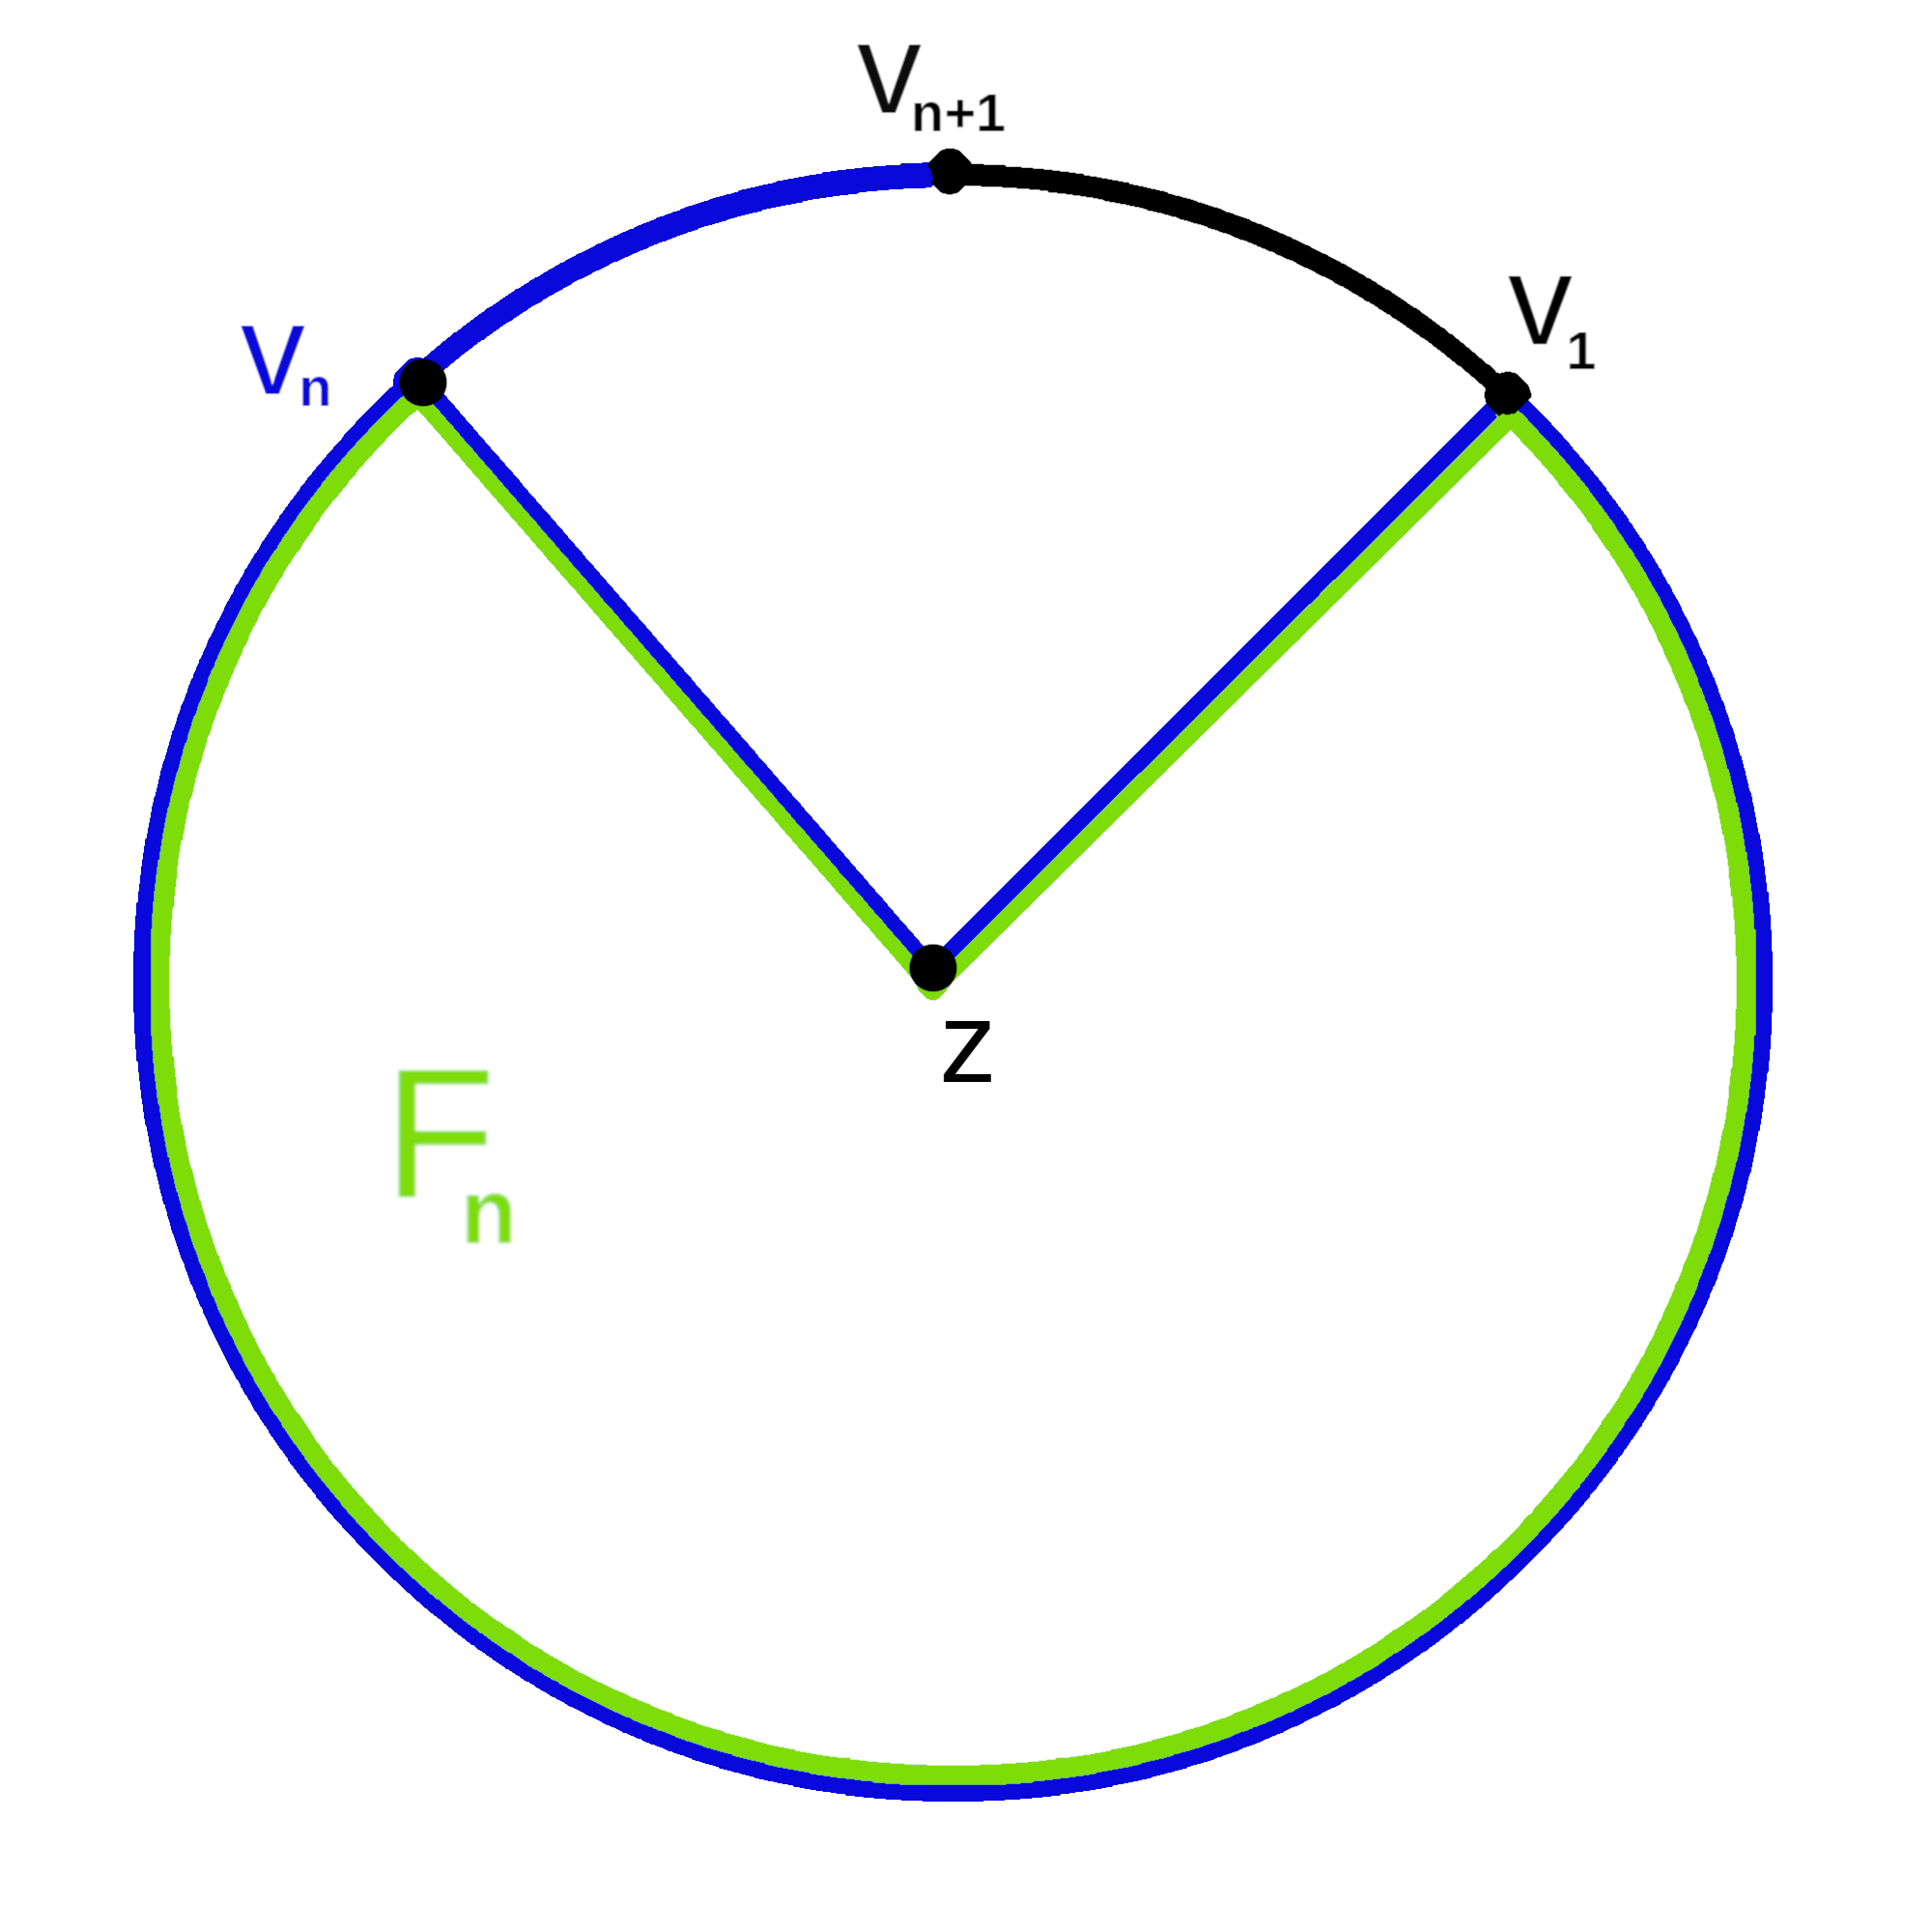
\includegraphics[width=1\textwidth]{klasse11.png}
        %\caption{In Klasse 1 sind die Spannbäume dieses Graphen, wobei die schwarze Kante in diesen Spannbäumen enthalten sein muss und der grün markierte Teil ein $F_n$ ist.}
        \captionof{figure}{In Klasse 1 sind die Spannbäume dieses Graphen, wobei die schwarze Kante in diesen Spannbäumen enthalten sein muss und der grün markierte Teil ein $F_n$ ist.}
 \label{klasse1} %caption vor label unbedingt
    \end{minipage}\hfill
    \begin{minipage}{0.45\textwidth}
        \centering
        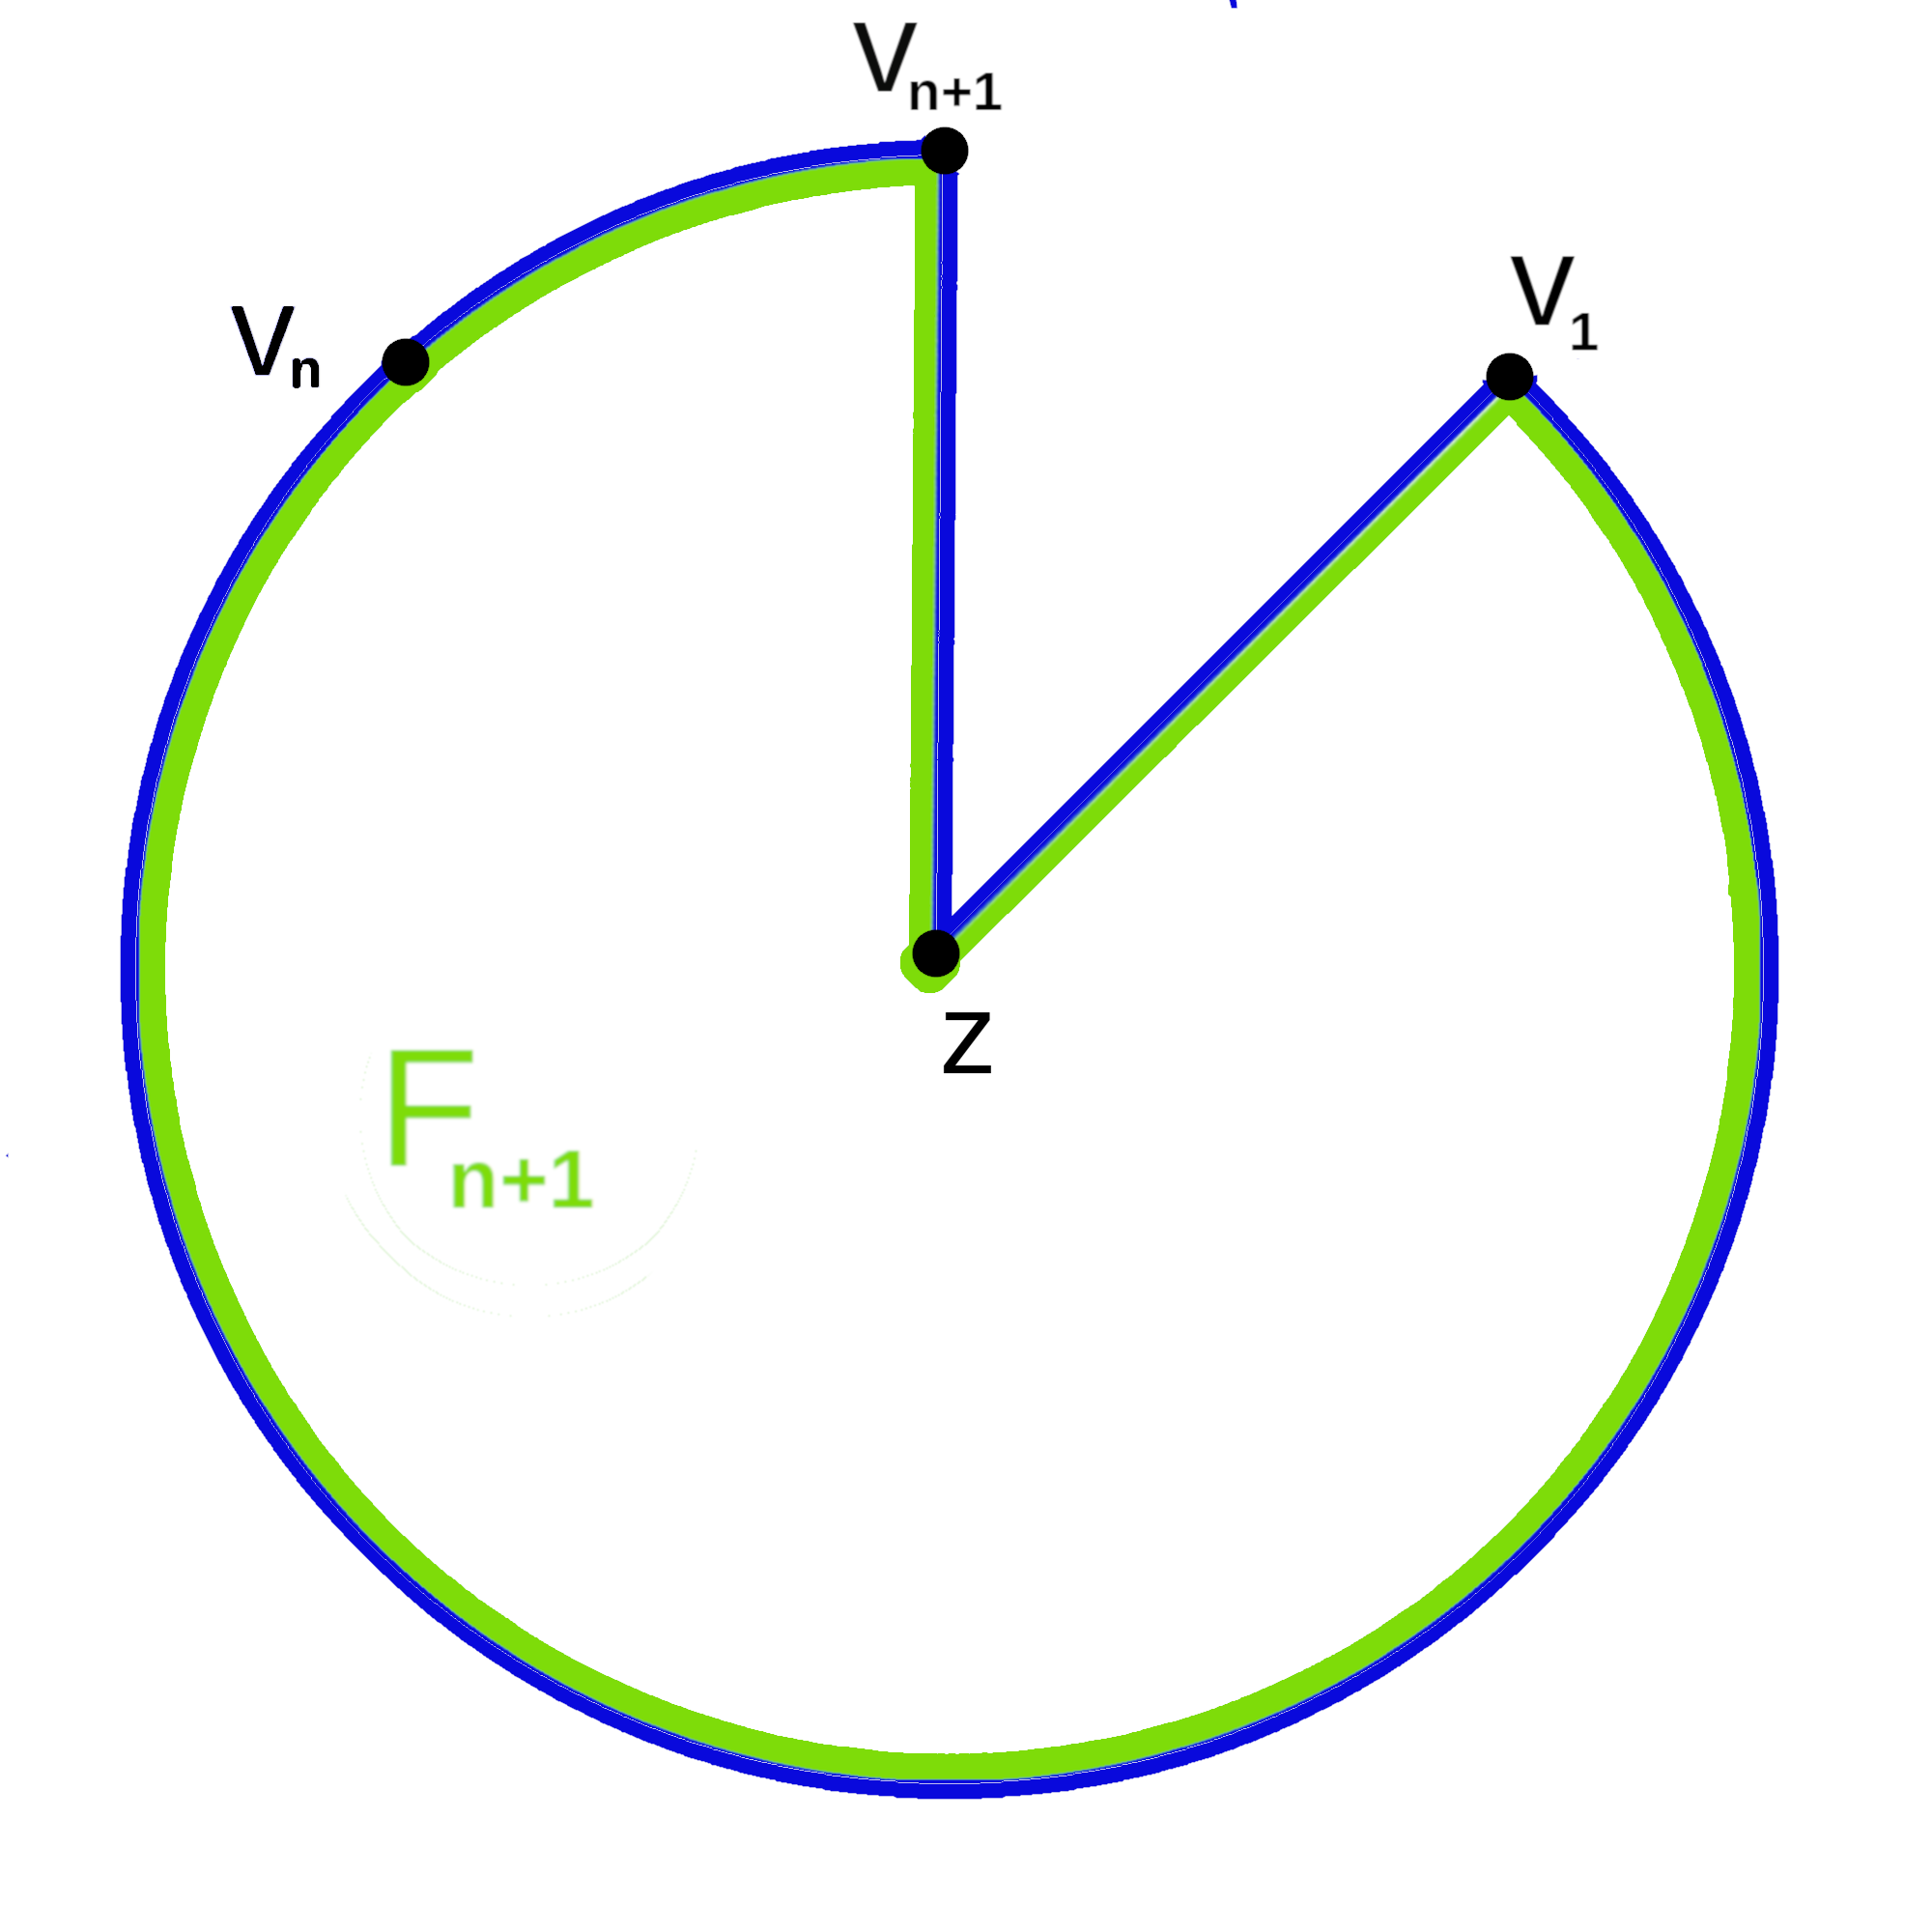
\includegraphics[width=1\textwidth]{klasse22.png}
        %\caption{In Klasse 2 sind genau die Spannbäume dieses Graphen, wobei der grün markierte Teil ein $F_{n+1}$ ist.}
        \captionof{figure}{In Klasse 2 sind genau die Spannbäume dieses Graphen, wobei der grün markierte Teil ein $F_{n+1}$ ist.}
 \label{klasse2} %caption vor label unbedingt
    \end{minipage}
%\end{figure}
\vspace{1cm}

Um zu zeigen dass die Klasse 3 genausoviele Spannbäume enthält wie $F_n$, werden wir beweisen, dass für die Anzahl der Spannbäume in Klasse 3 den gleichen rekursiven Formeln genügen, wie die von $F_n$.\\
Sei $a_n$ die Anzahl der Subgraphen von $F_n$, die aus genau zwei Komponenten bestehen, von denen eine den Knoten $z$ und die andere $v_n$ enthält.\\
Wir definieren $b_n$ als die Anzahl der Spannbäume in Klasse 3, die die Kanten $v_nv_{n+1}$ und $v_nz$ nicht enthalten.\\
Wir beweisen zuerst, dass $\mathit{k}\left(F_{n+1}\right)=2\mathit{k}\left(F_{n}\right)+a_n$ für $n\geq 2$.
Dazu nehmen wir ohne Beschränkung der Allgemeinheit an, dass $v_{n+1}$ nur zu den Knoten $v_n$ und $z$ adjazent ist. Ein Spannbaum des $F_n+1$ ist dann entweder durch hinzufügen einer der beiden Kanten $v_nv_{n+1}$ und $v_{n+1}z$ entstanden, oder durch hinzufügen beider Kanten an einen Subgraphen von $F_n$, der aus genau zwei Komponenten besteht, von denen eine den Knoten $z$ und die andere $v_n$ enthält.\\
Es gilt also $\mathit{k}\left(F_{n+1}\right)=2\mathit{k}\left(F_{n}\right)+a_n$.\\
Jetzt betrachten wir die Spannbäume aus Klasse 3.\\
Sei $M_n$ die Menge der Spannbäume von $W_{n+1}$ aus Klasse 3;\\
Nun zeigen wir, dass für $n \geq 3$ $|M_{n+1}|=2|M_n|+b_n$ ist.\\
Im folgenden betrachten wir nur $n \geq 3$. Wir erinnern uns an dieser Stelle daran, dass wir die Knoten beliebig umnummerieren können; in $M_{n+1}$ sind also die Spannbäume des Graphen aus Abbildung~\ref{mn1}.
\begin{figure}[H]
  \centering
 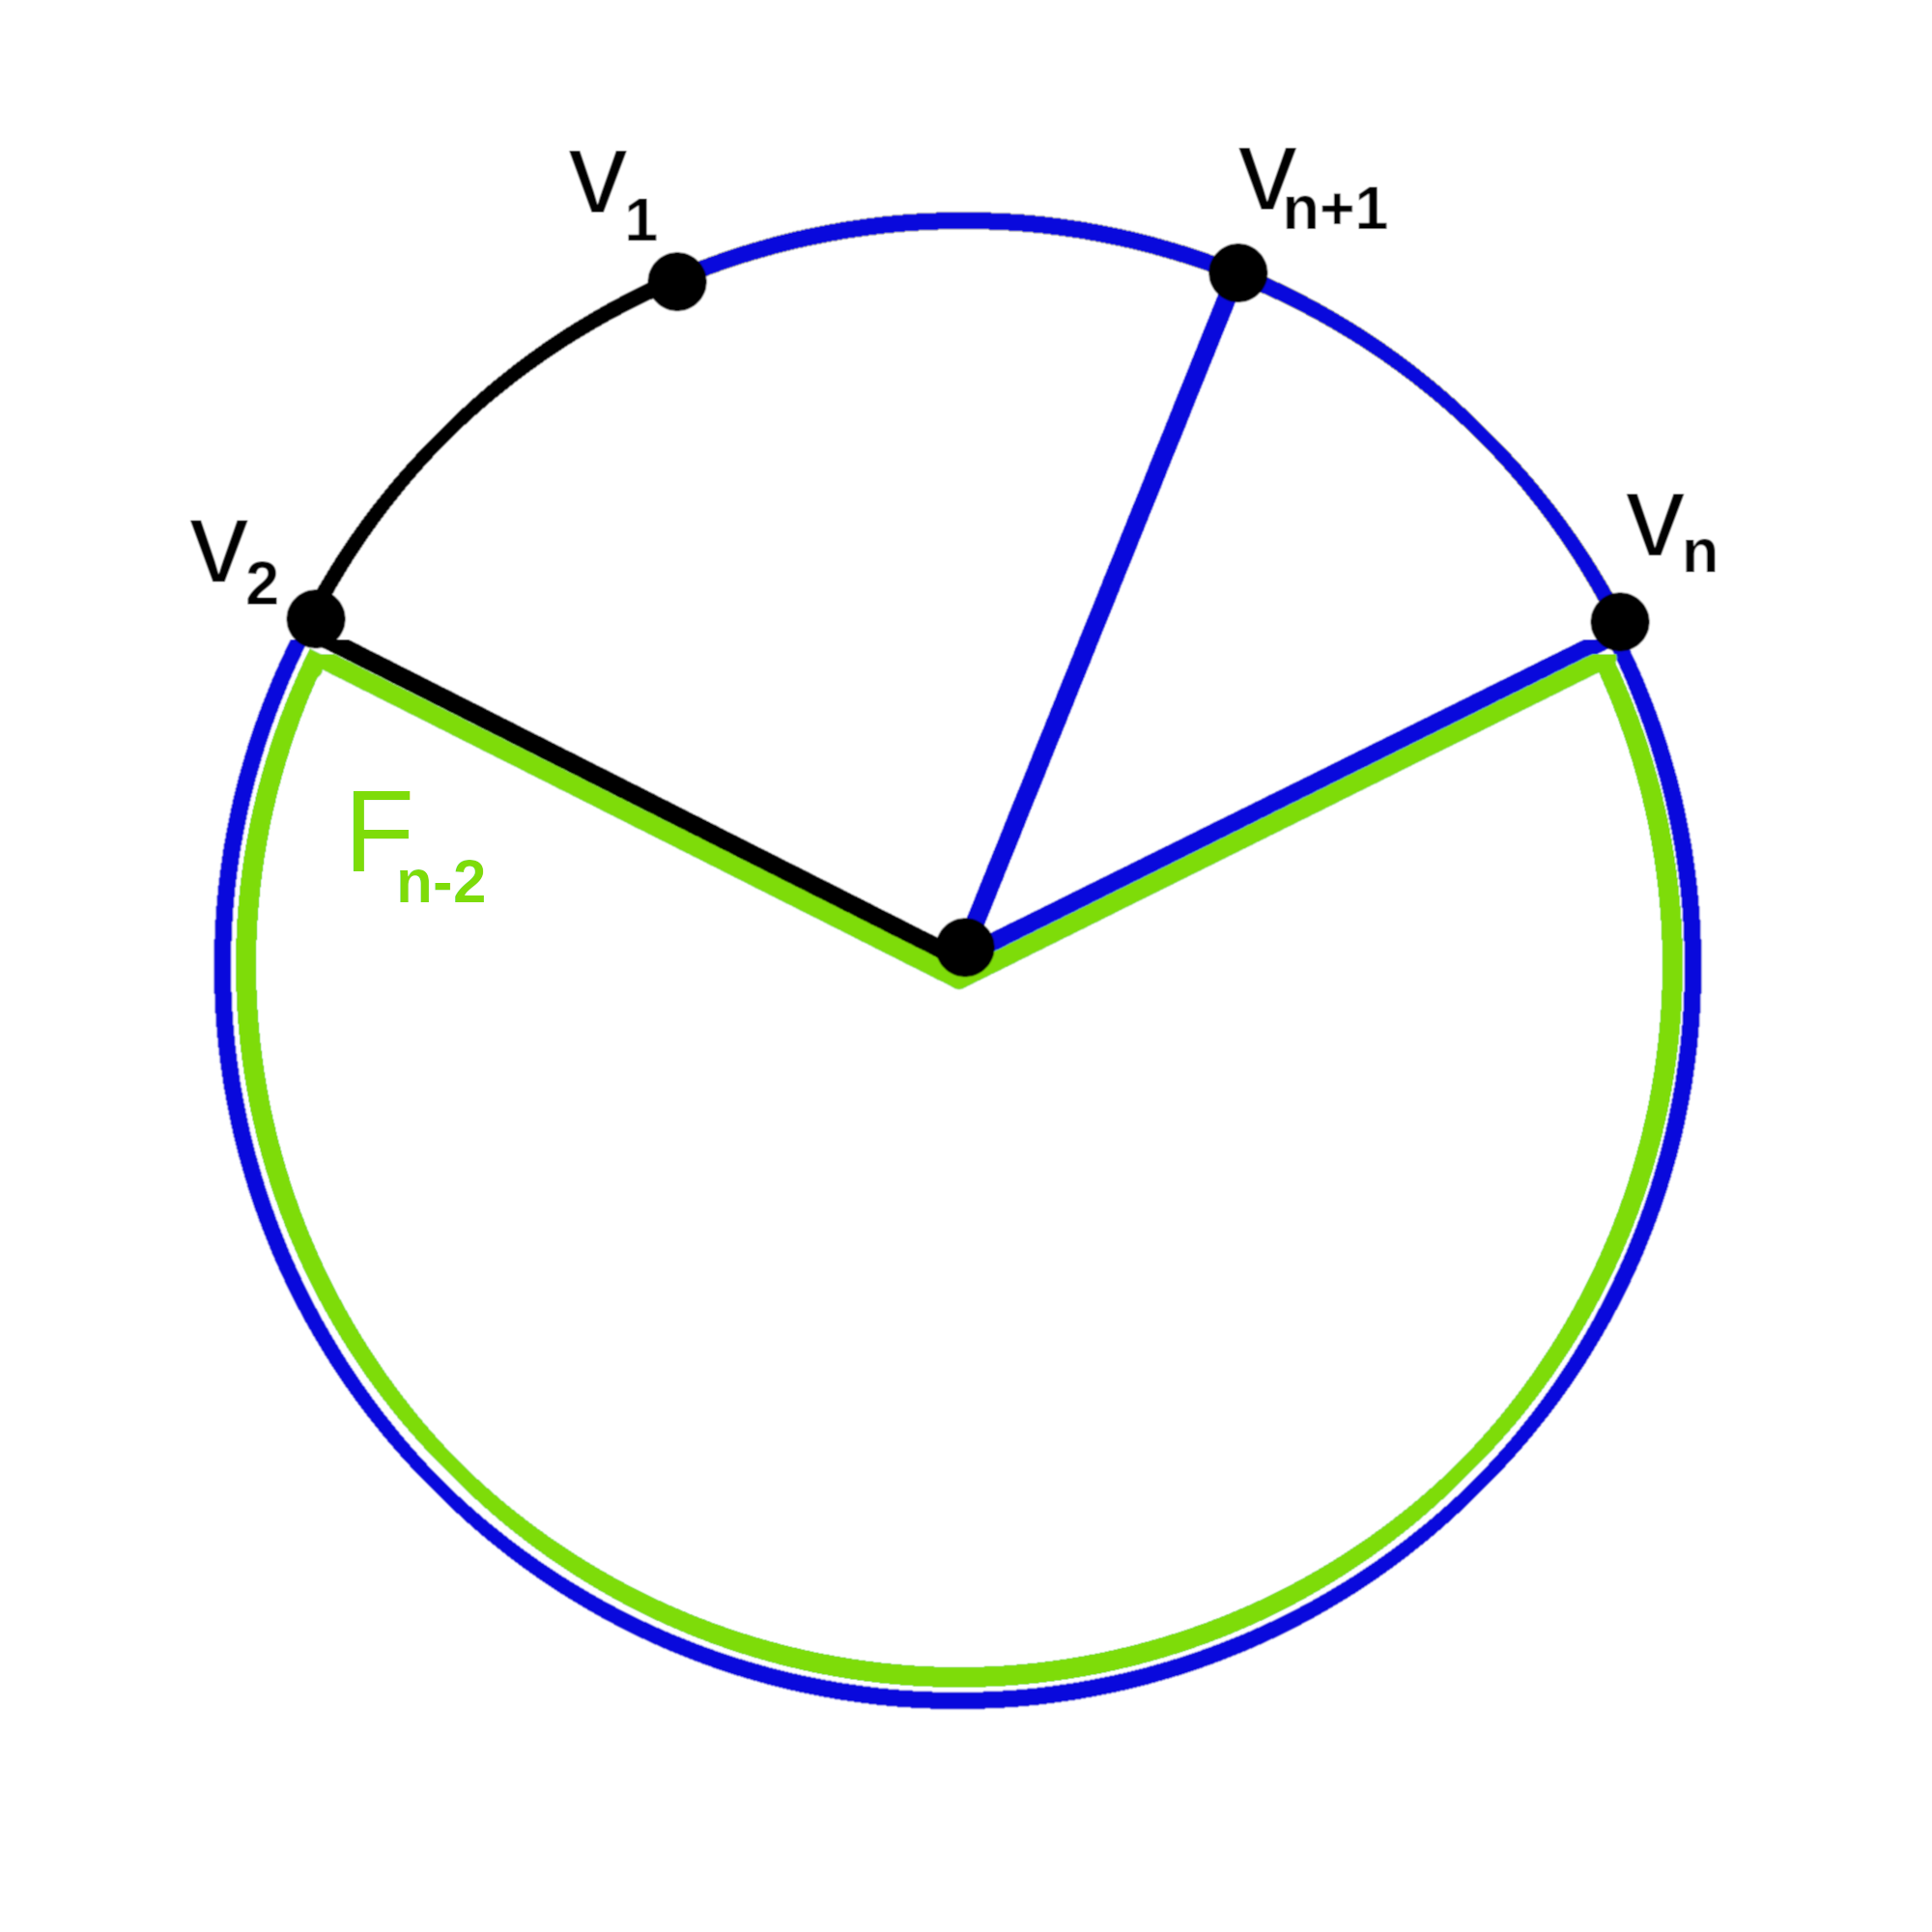
\includegraphics[width=0.5\textwidth]{mn1.png}
 \caption{}
 \label{mn1} %caption vor label unbedingt
\end{figure}
Wir unterteilen die Spannbäume davon auch in drei Klassen:\\
\par
\begingroup
\leftskip=20pt
\rightskip=20pt
\noindent
Die Erste bilden diejenigen, in denen die Kante $v_{n+1}z$ enthalten ist; Wie wir in der Abbildung~\ref{mn2} erkennen können, sind das soviele, wie in $M_n$.\\
Die Zweite besteht aus denen, die die Kante $v_nv_{n+1}$ enthalten; In Abbildung~\ref{mn3} sehen wir, dass das auch $|M_n|$ Stück sind.\\
Die Dritte beinhaltet die, die weder die Kante $v_{n+1}z$ noch die Kante $v_nv_{n+1}$ enthalten; die Anzahl davon ist nach Definition genau $b_n$.\\
\par
\endgroup
\begin{figure}[H]
    \centering
    \begin{minipage}{0.45\textwidth}
        \centering
        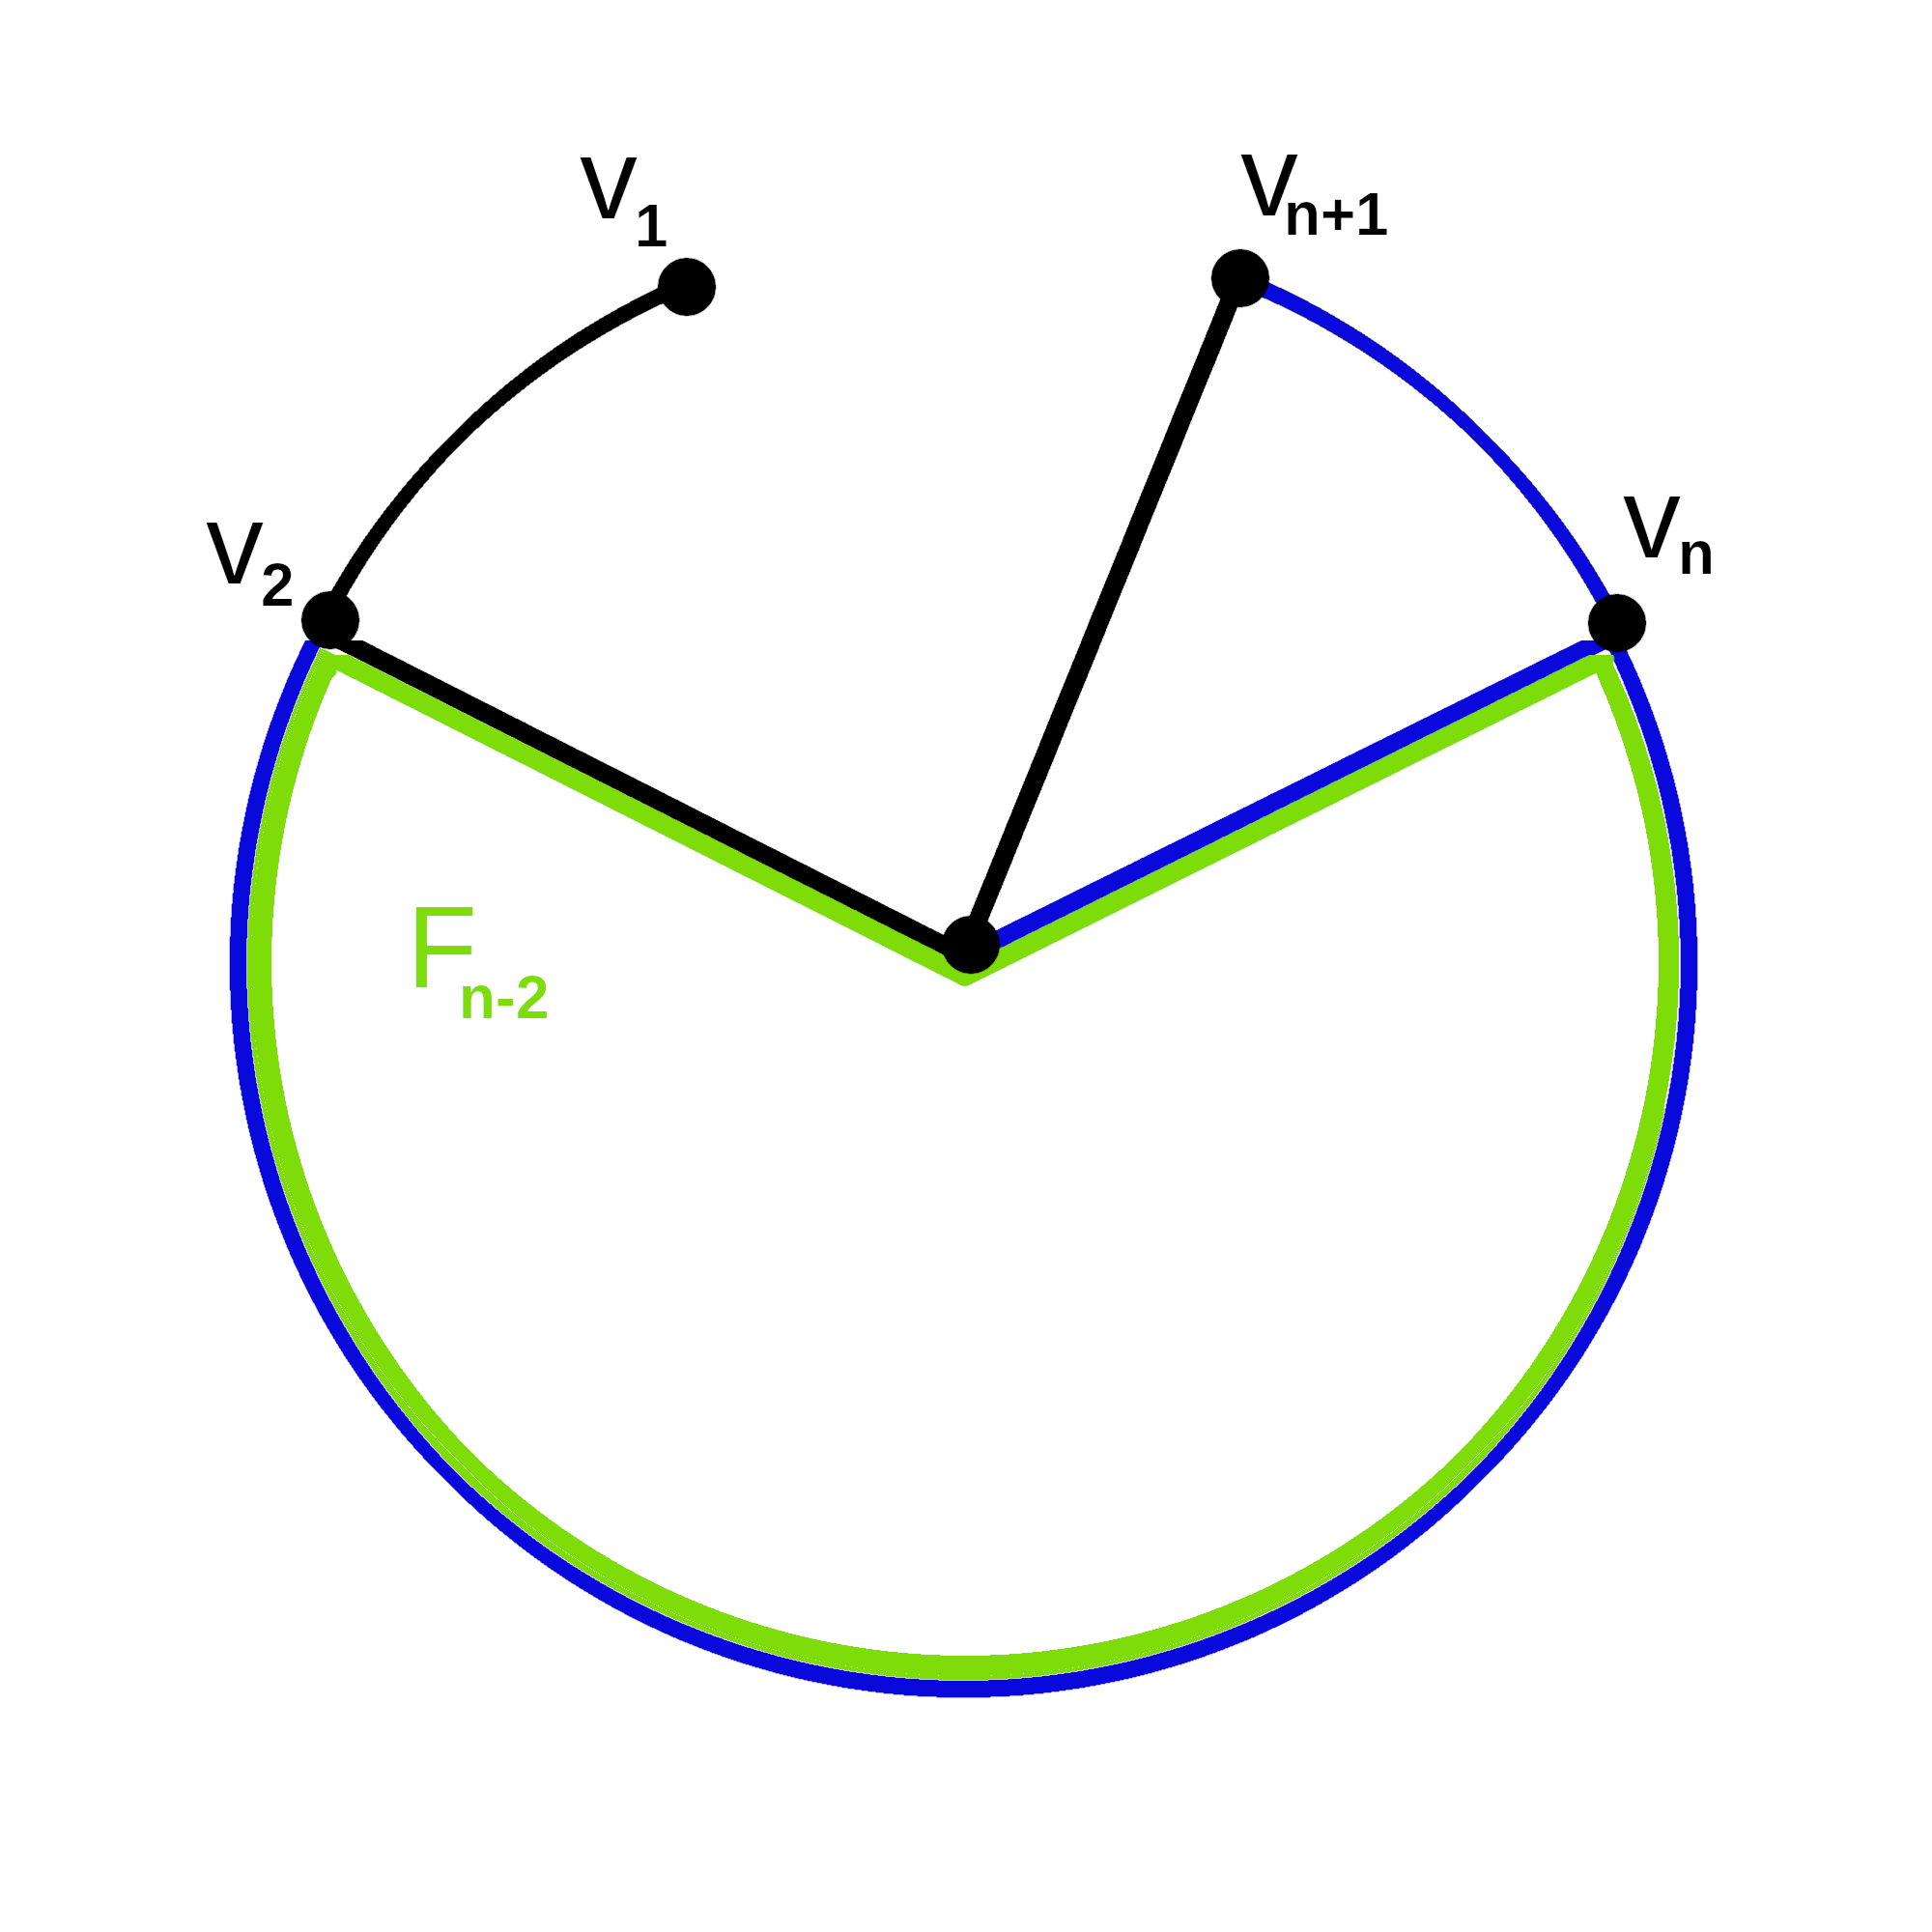
\includegraphics[width=1\textwidth]{mn2.png}
        \caption{}
 \label{mn2} %caption vor label unbedingt
    \end{minipage}\hfill
    \begin{minipage}{0.45\textwidth}
        \centering
        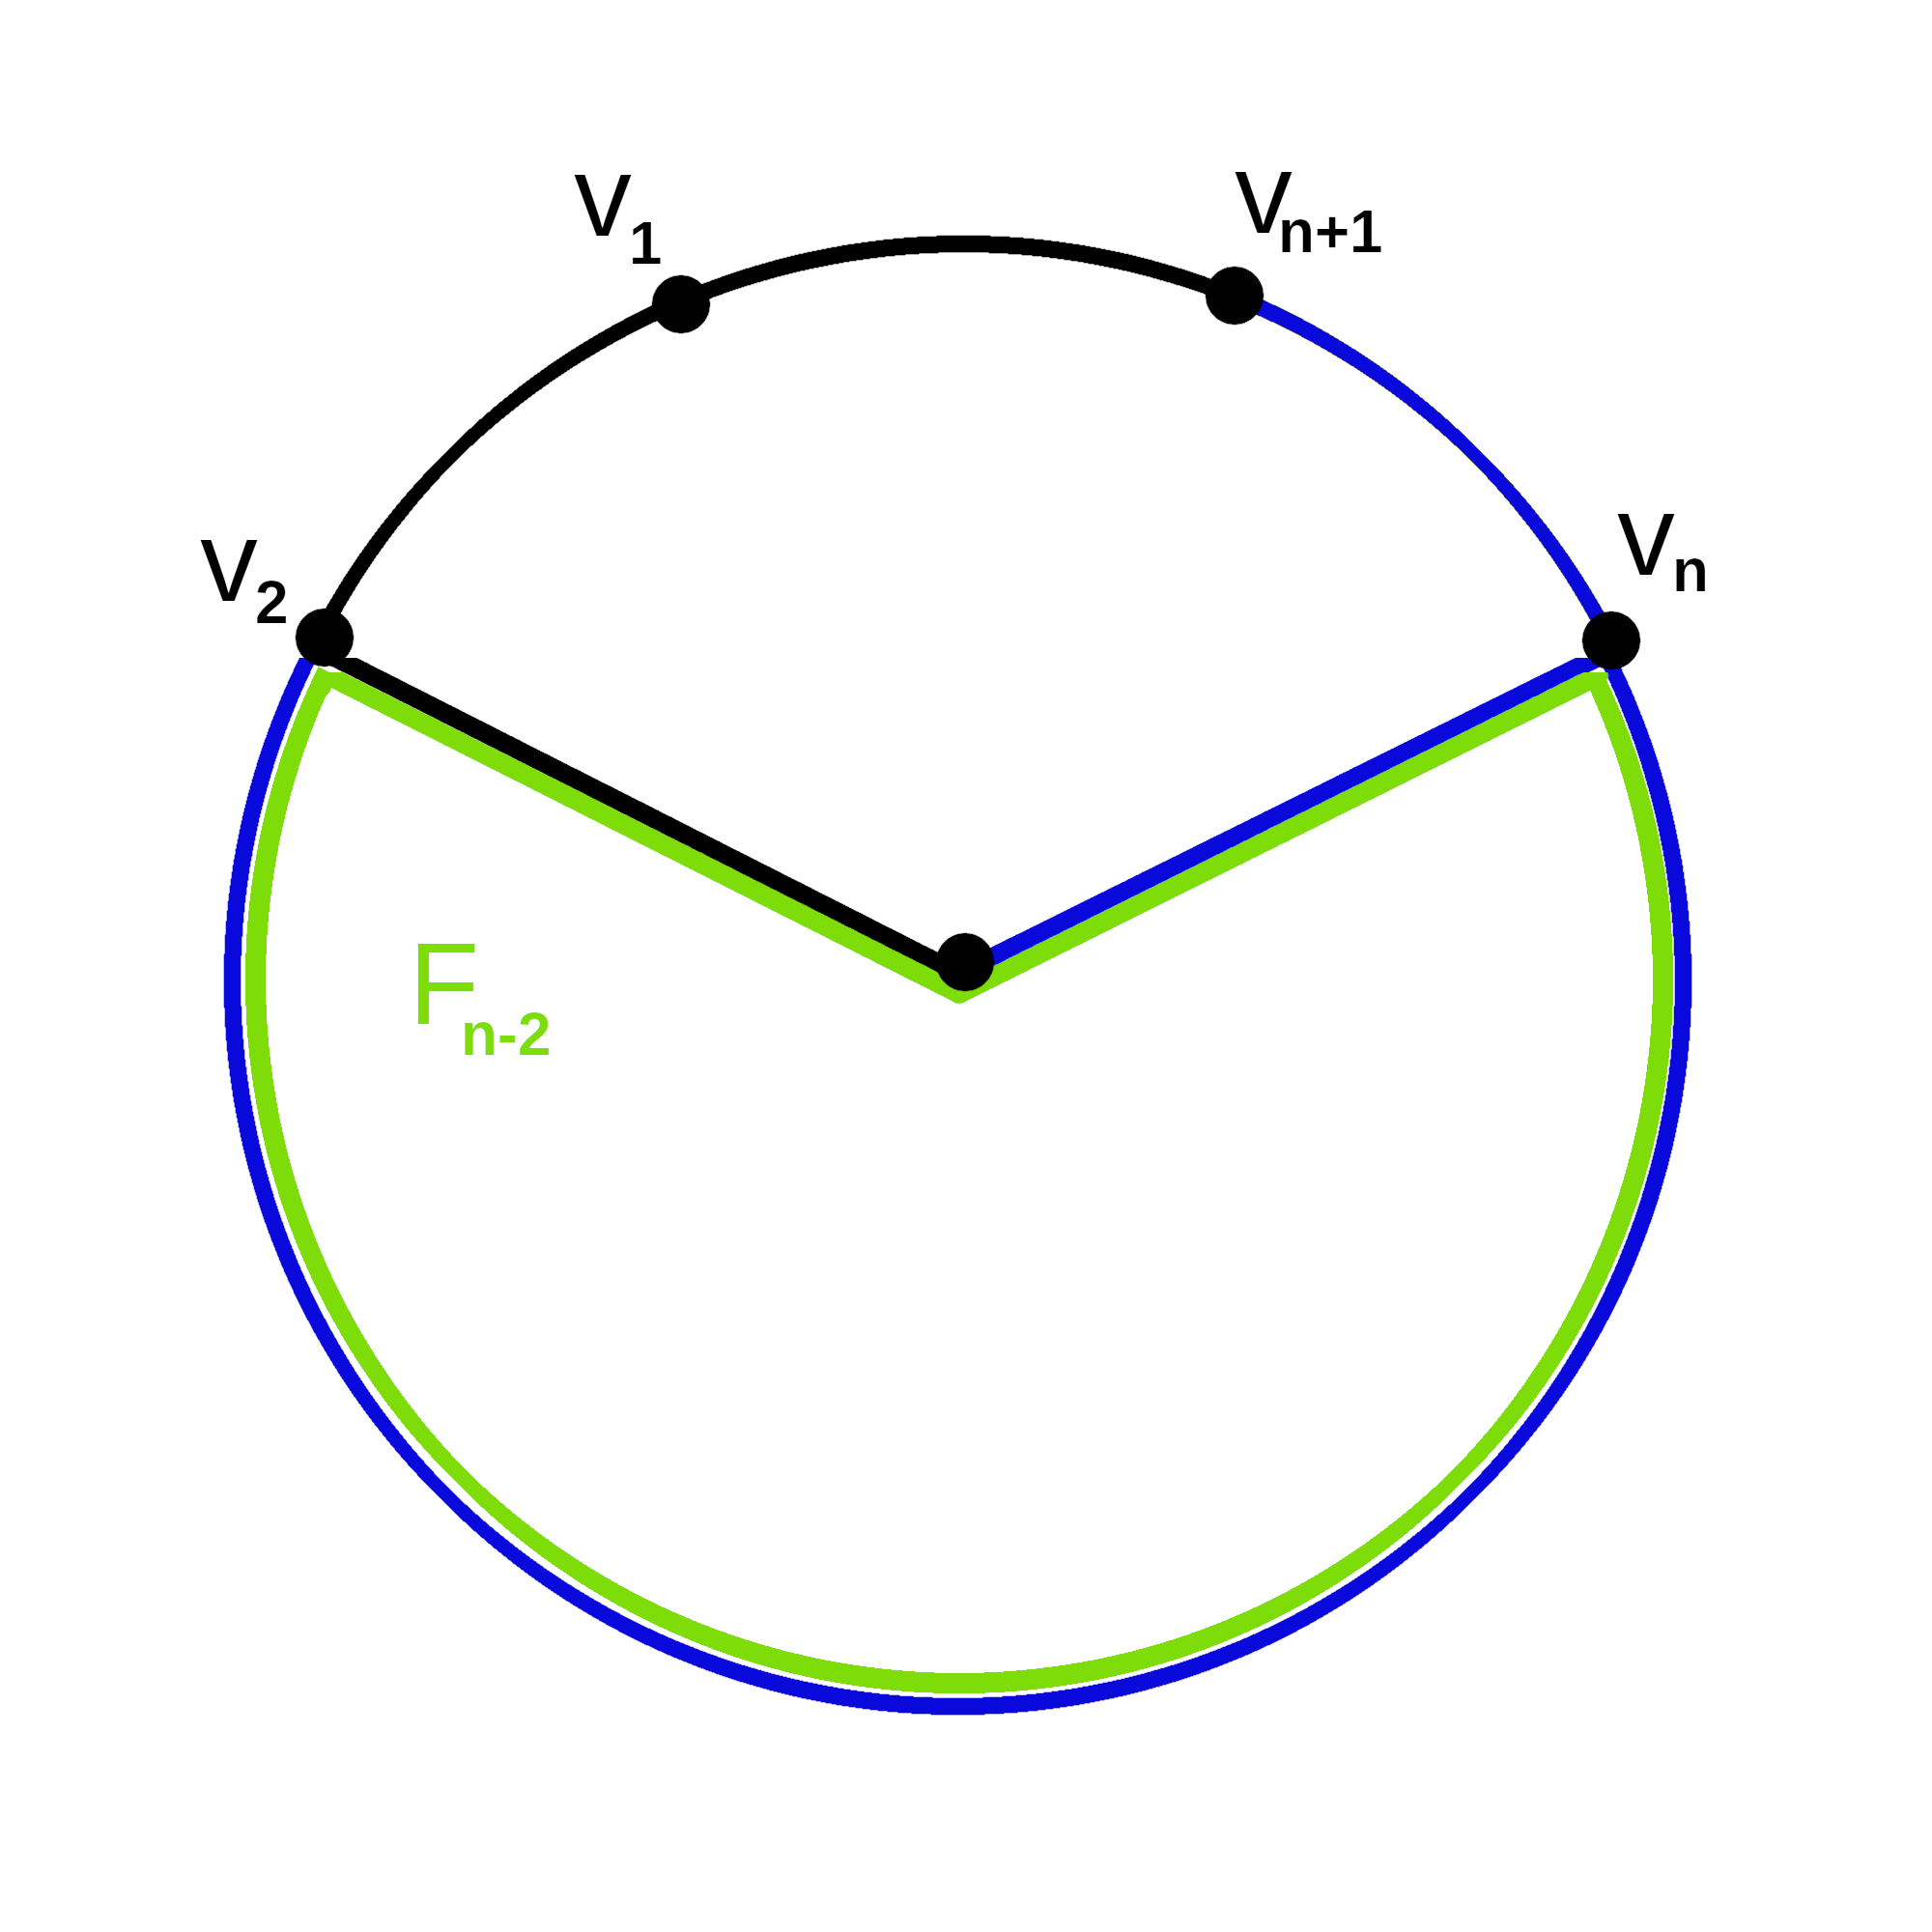
\includegraphics[width=1\textwidth]{mn3.png}
        \caption{}
 \label{mn3} %caption vor label unbedingt
    \end{minipage}
\end{figure}
Daraus schließen wir also $|M_{n+1}|=2|M_n|+b_n$ für $n\geq3$.\\
Wir sehen leicht, dass $\mathit{k}\left(F_2\right) = |M_2|$, $\mathit{k}\left(F_2\right)=|M_3|$ $a_2=b_2$ und $a_3=b_3$; daraus schließen wir, dass die Anzahl der Spannbäume in Klasse 3 gleich $\mathit{k}\left(F_{n}\right)$ ist, was wir zeigen wollten.\\
Da jeder Spannbaum von $W_{n+1}$ in genau einer der 3 Klassen ist, gilt die rekursive Beziehung
\begin{equation}
\mathit{k}\left(W_{n+1}\right) = \mathit{k}\left(F_{n+1}\right) + \mathit{k}\left(F_n\right) + \mathit{k}\left(W_n\right)
\label{eq:wrek}
\end{equation}
Wir werden nun den Beweis per Induktion über $n \in \mathbb{N}, \, n \geq 3$ vervollständigen, wobei uns natürlich zu Gute kommt, dass uns die Anzahl der Spannbäume von Fan-Graphen schon bekannt ist.\\
Für unseren Induktionsanfang sehen wir -zum Beispiel durch Anwendung von Kirchhoffs Matrix-Tree-Theorem- leicht, dass \begin{equation}
\mathit{k}\left(W_3\right) = 16 = \left(\frac{3+\sqrt{5}}{2}\right)^3+\left(\frac{3+\sqrt{5}}{2}\right)^3-2.
\end{equation}
Wir nehmen nun an, dass für ein $n \in \mathbb{N}$ die Formel 
\begin{equation}
 \mathit{k}\left(W_n\right) = \left(\frac{3+\sqrt{5}}{2}\right)^n+\left(\frac{3+\sqrt{5}}{2}\right)^n-2
\end{equation}
gilt.\\
Damit bleibt noch zu zeigen, dass
\begin{equation}
 \mathit{k}\left(W_{n+1}\right) = \left(\frac{3+\sqrt{5}}{2}\right)^{n+1}+\left(\frac{3+\sqrt{5}}{2}\right)^{n+1}-2.
\end{equation}
Das werden wir nun einfach ausrechnen.
Nachdem wir im vorherigen Kapitel herausgefunden haben, wieviele Spannbäume Fan-Graphen haben, setzen wir das und unsere Induktionsannahme in die Gleichung (\ref{eq:wrek}) ein, und erhalten:\\
\begin{equation}
\begin{aligned}
\mathit{k}\left(W_{n+1}\right) ={} & \frac{\left(3+\sqrt{5}\right)^{n+1}-\left(3-\sqrt{5}\right)^{n+1}}{2^{n+1}\sqrt{5}} + \frac{\left(3+\sqrt{5}\right)^{n}-\left(3-\sqrt{5}\right)^{n}}{2^{n}\sqrt{5}}\\
& + \left(\frac{3+\sqrt{5}}{2}\right)^n+\left(\frac{3-\sqrt{5}}{2}\right)^n-2
\end{aligned}
\end{equation}
Wir bringen fast alles auf einen Nenner, sortieren die Terme und bekommen
\begin{equation}
\begin{aligned}
\mathit{k}\left(W_{n+1}\right) = {}  & \frac{\left(3+\sqrt{5}+2+2\sqrt{5}\right)\left(3+\sqrt{5}\right)^{n}}{2^{n+1}\sqrt{5}} \\%% {} steht da nur, weils hin muss, wegen dem =
                        & -\frac{\left(3+\sqrt{5}+2-2\sqrt{5}\right)\left(3-\sqrt{5}\right)^{n}}{2^{n+1}\sqrt{5}}-2 
\end{aligned}
\end{equation}
\todo[inline]{evtl. zusammengehörige Terme evtl. farbig markieren}
Ausrechnen führt uns zu\\
\begin{equation}
\mathit{k}\left(W_{n+1}\right) = \left(\frac{3+\sqrt{5}}{2}\right)^{n+1}+\left(\frac{3+\sqrt{5}}{2}\right)^{n+1}-2
\end{equation}
Damit ist unser Induktionsbeweis abgeschlossen und wir haben gezeigt, dass unser Satz \ref{wn} über die Anzahl der Spannbäume in einem Rad gilt.
\begin{flushright} $\Box$ \end{flushright} 

\subsection{Zirkuläre Graphen}
%Wo treten die auf (z.B. Circulant Graphs sind Cayley-Graphen zyklischer Gruppen)
Im Kapitel Warm-up ist uns schon ein zirkulärer Graph begegnet; der Kreis-Graph.\\
Wir nennen einen Graphen zirkulär (engl. "circulant") mit $n$ Knoten, wenn für $n \in \mathbb{N}$ und eine Menge $I \subset{\{1,..,\lfloor \frac{n}{2} \rfloor \}}\subset{\mathbb{N}}$ gilt, dass jeder Knoten $v$ genau zu jedem Knoten $(v+i) (\mod{n})$ mit $i \in I$ benachbart ist; wir bezeichnen solch einen Graphen kurz mit $C_n^I$.\\
\todo[inline, color=blue]{Im folgenden Satz nachm Leerzeichen einfügen dieselben zwischen nxn und Matrix wieder wegmachen, das gehört nämlich zusammen}
Wir erinnern uns, dass eine $n\times n$-Matrix zyklisch genannt wird, falls jede Spalte aus der vorherigen durch Anwendung der Permutation $(1...n)$ hervorgeht.\\
Das ist bei den Adjazenz- und Laplacematrizen von zirkulären Graphen, aufgrund dessen, wann Knoten benachbart sind, der Fall.\\
Zu Gute kommt uns das bei der Berechnung der Anzahl von Spannbäumen in zirkulären Graphen, denn die Eigenwerte einer zyklischen Matrix sind wohlbekannt.\\
Wir wollen in diesem Zusammenhang folgendes zeigen:
\begin{Tms}
Für die Anzahl der Spannbäume in zusammenhängenden zirkulären Graphen von Grad $d$ gilt:\\
\begin{equation}
\mathit{k}\left( C_n^I \right) = 
 \begin{cases}
\frac{1}{n} \prod_{j=1}^{n-1} \left(4 \sum_{k \in I} \sin^2 \left( \frac{kj\pi}{n}\right) \right)\qquad\qquad\qquad\qquad\quad\; ,\,falls\,\,\,d\,\,\,gerade\,ist\\
\frac{1}{n} \prod_{j=1}^{n-1} \left(4 \sum_{k \in I/\mathrm{sup}(I)} \sin^2 \left( \frac{kj\pi}{n}\right)-(-1)^j+1\right)\qquad,\,falls\,\,\,d\,\,\,ungerade\,ist
\end{cases}
\end{equation}
\label{tmc}
\end{Tms}
\textbf{Beweis:}\\
Wir beweisen den Satz ähnlich wie~\cite{wang_yang_1984}, berechnen daher die Eigenwerte der Laplacematrix und wenden danach Kirchhoffs Matrix-Tree-Theorem an.\\
Für unseren Graphen $C_n^I$ ist die Laplacematrix zirkulär; wir können sie also durch die erste Spalte eindeutig beschreiben. Der erste Eintrag ist $|I|$, die Einträge $(i+1)$  und $(n-i)$ sind $-1$ für $i \in I$, die übrigen $0$.\\
Des weiteren ist sind die Eigenwerte von zirkulären Matrizen ein bekanntes Resultat aus der linearen Algebra:
\begin{equation}
 \lambda_j = \sum_{k=1}^{n}l_k\mathrm{exp}{\left(\frac{2\pi \mathrm{i}j}{n}\right)}, \,\,\,\,\, {j\in\{0,\ldots,n-1\}}
\end{equation}
$l_k$ ist hier der $k$-te Eintrag der ersten Spalte.\\ 
Der Eigenwert $\lambda_0 = 0$. Da der Graph zusammenhängend ist, sind die übrigen Eigenwerte ungleich $0$ und mit Kirchhoffs Matrix-Tree-Theorem folgt:
\begin{equation}
 \mathit{k}(C_n^I)=\prod_{j=1}^{n-1} \lambda_j
\end{equation}
An dieser Stelle machen wir die Fallunterscheidung, ob der Graph geraden Grad hat, oder nicht.\\
\par
\begingroup
\leftskip=20pt
\rightskip=20pt
\noindent
\textbf{Fall 1:} Grad gerade; das heißt der Grad ist gleich $2|I|$\\
Dann ist für alle $j \in \{1,\ldots,n-1\}$
\begin{equation}
\begin{aligned}
 \lambda_j = {} & {2|I| - \left( \sum_{k\in I}\left(\mathrm{exp}{\left(\frac{2\pi \mathrm{i}jk}{n}\right)} + \mathrm{exp}{\left(\frac{2\pi \mathrm{i}j(n-k)}{n}\right)}\right)\right)}\\
 = {} & {\left( \sum_{k\in I}\left(\mathrm{exp}{\left(\frac{2\pi \mathrm{i}jk}{n}\right)} - 2 + \mathrm{exp}{\left(\frac{2\pi \mathrm{i}j(n-k)}{n}\right)}\right)\right)}\\
 = {} &-\left( \sum_{k\in I}\left(\mathrm{exp}{\left(\frac{\pi \mathrm{i}jk}{n}\right)} - \mathrm{exp}{\left(\frac{\pi \mathrm{i}j(n-k)}{n}\right)}\right)^2\right)\\
 ={} & 4\sum_{k\in I} \sin^2 \left( \frac{kj\pi}{n}\right)
 \end{aligned}
\end{equation}
,wobei wir die berühmte eulersche Formel verwendet haben.\\
\\ \textbf{Fall 2:} Grad ungerade; das bedeutet der Grad ist $2(|I|-1) + 1$\\
Dann gilt für alle $j \in \{1,\ldots,n-1\}$
\small
\begin{equation}
\begin{aligned}
 \lambda_j = {} & { 2(|I|-1)+1 - \left(\mathrm{exp}{\left(\frac{2\pi \mathrm{i}j \mathrm{sup}(I)}{n}\right)}+ \sum_{k\in I/\mathrm{sup}(I)}\left(\mathrm{exp}{\left(\frac{2\pi \mathrm{i}jk}{n}\right)}+ \mathrm{exp}{\left(\frac{2\pi \mathrm{i}j(n-k)}{n}\right)}\right)\right)}\\
  = {} &1-\left(\mathrm{exp}{\left(\frac{\pi \mathrm{i}j \mathrm{sup}(I)}{n}\right)} +\sum_{k\in I/\mathrm{sup}(I)}\left(\mathrm{exp}{\left(\frac{\pi \mathrm{i}jk}{n}\right)} - \mathrm{exp}{\left(\frac{\pi \mathrm{i}j(n-k)}{n}\right)}\right)^2\right)\\
  = {} & 4\sum_{k\in I/\mathrm{sup}(I)} \sin^2 \left( \frac{kj\pi}{n}\right)-(-1)^j+1
 \end{aligned}
\end{equation}
\normalsize
Hier sind wir wieder genauso vorgegangen, wie oben.\\
\par
\endgroup
Jetzt kennen wir die Eigenwerte der Laplacematrix, können Kirchhoffs Matrix-Tree-Theorem anwenden und es folgt
\begin{equation}
\mathit{k}\left( C_n^I \right) = 
 \begin{cases}
\frac{1}{n} \prod_{j=1}^{n-1} \left(4 \sum_{k \in I} \sin^2 \left( \frac{kj\pi}{n}\right) \right)\qquad\qquad\qquad\qquad\quad\; ,\,falls\,\,\,d\,\,\,gerade\,ist\\
\frac{1}{n} \prod_{j=1}^{n-1} \left(4 \sum_{k \in I/\mathrm{sup}(I)} \sin^2 \left( \frac{kj\pi}{n}\right)-(-1)^j+1\right)\qquad,\,falls\,\,\,d\,\,\,ungerade\,ist
\end{cases}
\end{equation}
Das wollten wir zeigen.
\begin{flushright} $\Box$ \end{flushright} 
\begin{Bsps}[$C_n^2$ - Das Quadrat eines Kreises]
\todo[inline, color=green]{Bild von einem Square of a cycle}
\todo[inline]{Herleitung Formel}
%Im Notfall einen anderen Beweis für $C_n^{(1,2)}$ raussuchen (eher nicht), der jetzige ist lang, allerdings nutzt er er das MTT was von Vorteil ist (ich werde die Rechnungen verkürzen und nur die wichtigen Teile ausführlich machen, sonst werden das 4-6 Seiten quasi nur mit Rechnungen)
\end{Bsps} 

\subsection{Kartesische Produkte von Graphen}
In diesem Teil zeigen wir, was im Bezug auf die Anzahl der Spannbäume geschieht, wenn man das kartesische Produkt von Graphen bildet.\\
Das kartesische Produkt $G_1\times G_2$ zweier Graphen $G1=(V_1,E_1)$ und $G2=(V_2,E_2)$ bezeichnet dabei den Graphen mit Knotenmenge $V_1\times V_2$ und Kantenmenge $(E_1\times V_2)\cup(V_1\times E_2)$, wobei zwei Knoten $(u_1,u_2), (v_1,v_2) \in (V_1\times V_2)$ genau dann in $G_1\times G_2$ benachbart sind, wenn entweder $u_1=v_1$ in $G_1$ oder $u_2=v_2$ in $G_2$ ist.\\
\todo[inline, color=yellow]{Ich werde wahrscheinlich ein/zwei Beispiele davon zeigen, z.B. Lattice-Graph, aber nicht mehr, weil das im Grund genommen einfach nur Rechnungen sind und das Matrix-Tree-Theorem nicht mehr als solches angewendet wird, sondern nur über den Satz unten(passt das?)---Antwort:JA->warmup-kapitel}
\todo[inline, color=yellow]{Vielleicht ist es sinnvoll ein weiteres Kapitel mit einfachen Graphen wie Kreis-Graphen, Pfad-Graphen,etc. zu machen, dann könnte man sich in diesem Kapitel fast alle Rechnungen  ersparen und nur ein/zwei Beispiele geben, was man daraus "basteln" kann (Gute Idee?)---Antwort:JA}
\begin{Tms}
 Sei $G$ ein Graph mit $m$ Knoten und Eigenwerten $\mu_1(G),..,\mu_m(G)$ und $H$ ein Graph mit $n$ Knoten und Eigenwerten $\mu_1(H),..,\mu_n(H)$. \\
% Dann sind die Eigenwerte des kartesischen Produkts $G \times H$ genau $\mu_i(G)+\mu_j(H)$ mit $i \in \{ 1,..,m\}, j \in \{ 1,..,n\}$.
Dann hat der Graph $G \times H$ genau
\begin{equation}
\frac{1}{nm}\displaystyle\prod_{i,j}(\mu_i(G)+\mu_j(H))1_{\{\mu_i(G)+\mu_j(H)\neq0\}}
\end{equation}
Spannbäume.
\end{Tms}
\textbf{Beweis:}\\
Für diesen Beweis werden wir die Gestalt der Laplacematrix von $G \times H$ ausnutzen und dann mithilfe der linearen Algebra Aussagen über die Eigenwerte treffen.\\
Wir beobachten, dass die Laplacematrix von $G\times H$ die Kroneckersumme der Laplacematrizen von $G$ und $H$ ist.\\
Aus der linearen Algebra wissen wir nun, dass die Eigenwerte der Kroneckersumme $L(G) \oplus L(H)$ genau $\mu_i(G)+\mu_j(H)$ mit $i \in \{ 1,..,m\}, j \in \{ 1,..,n\}$ sind.\\
Mit Kirchhoffs Matrix-Tree-Theorem folgt nun
\begin{equation}
 \mathit{k}(G \times H) = \frac{1}{nm}\displaystyle\prod_{i,j}(\mu_i(G)+\mu_j(H))1_{\{\mu_i(G)+\mu_j(H)\neq0\}}
\end{equation}
Damit ist unser Satz bewiesen.
\begin{flushright} $\Box$ \end{flushright} 
\todo[inline]{Beweis ganz sauber fertigmachen, evtl. Quelle in der man was über ide Kroneckersumme nachlesen kann}
\begin{Bsps}[Zylinder-Graph]
%pfad und kreis
\end{Bsps}
\begin{Bsps}[Torus-Graph]
kreis und Kreis
\end{Bsps}
\todo[inline, color=red]{Lattice Graph ist wieder Mehrdeutig, Gittergraph hier falsch}
\begin{Bsps}[kartesisches Produkt von vollständigen Graphen]
%z.B. rooks graph
\end{Bsps}
\todo[inline]{Bei den Beispielen werden wir vollstänige Graphen nutzen, da muss noch kurz argumentiert werden wie da die Eigenwerte sind}


%\graphicspath{{grafiken/}}

\chapter{Zusammenfassung}

Das in Abb.\,\ref{fig:LoremIpsum} beschriebene Verhalten charakterisiert die vorliegende Arbeit. Au\ss erdem sei an dieser Stelle auf Kap.\,\ref{chap:einleitung} verwiesen.

\begin{figure}[htbp]
\centering
\includegraphics[width=0.5\textwidth]{LoremIpsum}
\caption{Beschreibung des oben stehenden Bildes.}
\label{fig:LoremIpsum}
\end{figure}

An dieser Stelle will ich noch \cite{sahin:penning} zitieren, au\ss erdem ist in \cite{zibell:diplarbeit} gezeigt, dass es regnet \cite{zibell:phd}.

\cleardoublepage

\bibliography{bachelorarbeit}{}
\bibliographystyle{plain}

%\begin{appendix}
%\graphicspath{{grafiken/anhang/}}

\section{Zusatzinformationen}

Lorem ipsum dolor sit amet, consetetur sadipscing elitr, sed diam nonumy eirmod tempor invidunt ut labore et dolore magna aliquyam erat, sed diam voluptua. At vero eos et accusam et justo duo dolores et ea rebum. Stet clita kasd gubergren, no sea takimata sanctus est Lorem ipsum dolor sit amet. Lorem ipsum dolor sit amet, consetetur sadipscing elitr, sed diam nonumy eirmod tempor invidunt ut labore et dolore magna aliquyam erat, sed diam voluptua. At vero eos et accusam et justo duo dolores et ea rebum. Stet clita kasd gubergren, no sea takimata sanctus est Lorem ipsum dolor sit amet.


%\end{appendix}

\clearpage{\pagestyle{empty}\cleardoublepage}
%\cleardoublepage
\thispagestyle{empty}

\vspace*{1cm}
{\huge \textbf{Selbständigkeitserklärung}}\\
\vspace*{1.5cm}

Ich versichere hiermit, die vorliegende Arbeit mit dem Titel

\begin{center}
	\textbf{Das Matrix-Tree-Theorem}
\end{center}

selbständig verfasst zu haben und keine anderen als die angegebenen Quellen und Hilfsmittel verwendet zu haben.

\vspace*{3cm}

Christopher Mann

\vspace*{1cm}
München, den \myformat\today

\end{document}
